%% (Master) Thesis template
% Template version used: v1.4
%
% Largely adapted from Adrian Nievergelt's template for the ADPS
% (lecture notes) project.


%% We use the memoir class because it offers a many easy to use features.
\documentclass[11pt,a4paper,titlepage]{memoir}

%% Packages
%% ========

%% LaTeX Font encoding -- DO NOT CHANGE
\usepackage[OT1]{fontenc}

%% Babel provides support for languages.  'english' uses British
%% English hyphenation and text snippets like "Figure" and
%% "Theorem". Use the option 'ngerman' if your document is in German.
%% Use 'american' for American English.  Note that if you change this,
%% the next LaTeX run may show spurious errors.  Simply run it again.
%% If they persist, remove the .aux file and try again.
\usepackage[english]{babel}

%% Input encoding 'utf8'. In some cases you might need 'utf8x' for
%% extra symbols. Not all editors, especially on Windows, are UTF-8
%% capable, so you may want to use 'latin1' instead.
\usepackage[utf8]{inputenc}

%% This changes default fonts for both text and math mode to use Herman Zapfs
%% excellent Palatino font.  Do not change this.
\usepackage[sc]{mathpazo}

%% The AMS-LaTeX extensions for mathematical typesetting.  Do not
%% remove.
\usepackage{amsmath,amssymb,amsfonts,mathrsfs}

%% NTheorem is a reimplementation of the AMS Theorem package. This
%% will allow us to typeset theorems like examples, proofs and
%% similar.  Do not remove.
%% NOTE: Must be loaded AFTER amsmath, or the \qed placement will
%% break
\usepackage[amsmath,thmmarks]{ntheorem}

%% LaTeX' own graphics handling
\usepackage{graphicx}

%% We unfortunately need this for the Rules chapter.  Remove it
%% afterwards; or at least NEVER use its underlining features.
\usepackage{soul}

%% This allows you to add .pdf files. It is used to add the
%% declaration of originality.
\usepackage{pdfpages}

%% Some more packages that you may want to use.  Have a look at the
%% file, and consult the package docs for each.
%% See the TeXed file for more explanations

%% [OPT] Multi-rowed cells in tabulars
%\usepackage{multirow}

%% [REC] Intelligent cross reference package. This allows for nice
%% combined references that include the reference and a hint to where
%% to look for it.
\usepackage{varioref}

%% [OPT] Easily changeable quotes with \enquote{Text}
%\usepackage[german=swiss]{csquotes}

%% [REC] Format dates and time depending on locale
\usepackage{datetime}

%% [OPT] Provides a \cancel{} command to stroke through mathematics.
%\usepackage{cancel}

%% [NEED] This allows for additional typesetting tools in mathmode.
%% See its excellent documentation.
\usepackage{mathtools}

%% [ADV] Conditional commands
%\usepackage{ifthen}

%% [OPT] Manual large braces or other delimiters.
%\usepackage{bigdelim, bigstrut}

%% [REC] Alternate vector arrows. Use the command \vv{} to get scaled
%% vector arrows.
\usepackage[h]{esvect}

%% [NEED] Some extensions to tabulars and array environments.
\usepackage{array}

%% [OPT] Postscript support via pstricks graphics package. Very
%% diverse applications.
%\usepackage{pstricks,pst-all}

%% [?] This seems to allow us to define some additional counters.
%\usepackage{etex}

%% [ADV] XY-Pic to typeset some matrix-style graphics
%\usepackage[all]{xy}

%% [OPT] This is needed to generate an index at the end of the
%% document.
%\usepackage{makeidx}

%% [OPT] Fancy package for source code listings.  The template text
%% needs it for some LaTeX snippets; remove/adapt the \lstset when you
%% remove the template content.
\usepackage{listings}
\lstset{language=TeX,basicstyle={\normalfont\ttfamily}}

%% [REC] Fancy character protrusion.  Must be loaded after all fonts.
\usepackage[activate]{pdfcprot}

%% [REC] Nicer tables.  Read the excellent documentation.
\usepackage{booktabs}


%% Our layout configuration.  DO NOT CHANGE.
%% Memoir layout setup

%% NOTE: You are strongly advised not to change any of them unless you
%% know what you are doing.  These settings strongly interact in the
%% final look of the document.

% Dependencies
\usepackage{ITUlogo}
\usepackage{titlesec}

% Turn extra space before chapter headings off.
\setlength{\beforechapskip}{0pt}

\nonzeroparskip
\parindent=0pt
\defaultlists

% Chapter style redefinition
\makeatletter

\if@twoside
  \pagestyle{Ruled}
  \copypagestyle{chapter}{Ruled}
\else
  \pagestyle{ruled}
  \copypagestyle{chapter}{ruled}
\fi
\makeoddhead{chapter}{}{}{}
\makeevenhead{chapter}{}{}{}
\makeheadrule{chapter}{\textwidth}{0pt}
\copypagestyle{abstract}{empty}

\makechapterstyle{bianchimod}{%
  \chapterstyle{default}
  \renewcommand*{\chapnamefont}{\normalfont\Large\sffamily}
  \renewcommand*{\chapnumfont}{\normalfont\Large\sffamily}
  \renewcommand*{\printchaptername}{%
    \chapnamefont\centering\@chapapp}
  \renewcommand*{\printchapternum}{\chapnumfont {\thechapter}}
  \renewcommand*{\chaptitlefont}{\normalfont\huge\sffamily}
  \renewcommand*{\printchaptertitle}[1]{%
    \hrule\vskip\onelineskip \centering \chaptitlefont\textbf{\vphantom{gyM}##1}\par}
  \renewcommand*{\afterchaptertitle}{\vskip\onelineskip \hrule\vskip
    \afterchapskip}
  \renewcommand*{\printchapternonum}{%
    \vphantom{\chapnumfont {9}}\afterchapternum}}

% Use the newly defined style
\chapterstyle{bianchimod}

\setsecheadstyle{\Large\bfseries\sffamily}
\setsubsecheadstyle{\large\bfseries\sffamily}
\setsubsubsecheadstyle{\bfseries\sffamily}
\setparaheadstyle{\normalsize\bfseries\sffamily}
\setsubparaheadstyle{\normalsize\itshape\sffamily}
\setsubparaindent{0pt}

% Set captions to a more separated style for clearness
\captionnamefont{\sffamily\bfseries\footnotesize}
\captiontitlefont{\sffamily\footnotesize}
\setlength{\intextsep}{16pt}
\setlength{\belowcaptionskip}{1pt}

% Set section and TOC numbering depth to subsection
\setsecnumdepth{subsubsection}
\settocdepth{subsubsection}
\setcounter{secnumdepth}{4}
\titleformat{\paragraph}
{\normalfont\normalsize\bfseries}{\theparagraph}{1em}{}
\titlespacing*{\paragraph}
{0pt}{3.25ex plus 1ex minus .2ex}{1.5ex plus .2ex}

%% Titlepage adjustments
\pretitle{\vspace{0pt plus 0.7fill}\begin{center}\HUGE\sffamily\bfseries}
\posttitle{\end{center}\par}
\preauthor{\par\begin{center}\let\and\\\Large\sffamily}
\postauthor{\end{center}}
\predate{\par\begin{center}\Large\sffamily}
\postdate{\end{center}}

\def\@advisors{}
\newcommand{\advisors}[1]{\def\@advisors{#1}}
\def\@department{}
\newcommand{\department}[1]{\def\@department{#1}}
\def\@thesistype{}
\newcommand{\thesistype}[1]{\def\@thesistype{#1}}

\renewcommand{\maketitlehooka}{\par\begin{center}\ITUlogo[5in]\end{center}}

\renewcommand{\maketitlehookb}{\vspace{1in}%
  \par\begin{center}\Large\sffamily\@thesistype\end{center}}

\renewcommand{\maketitlehookd}{%
  \vfill\par
  \begin{flushright}
    \sffamily
    \@advisors\par
    \@department,\par Istanbul Technical University
  \end{flushright}
}

\checkandfixthelayout

\setlength{\droptitle}{-48pt}

\makeatother

% This defines how theorems should look. Best leave as is.
\theoremstyle{plain}
\setlength\theorempostskipamount{0pt}

%%% Local Variables:
%%% mode: latex
%%% TeX-master: "thesis"
%%% End:


%% Theorem environments.  You will have to adapt this for a German
%% thesis.
%% Theorem-like environments

%% This can be changed according to language. You can comment out the ones you
%% don't need.

\numberwithin{equation}{chapter}

%% German theorems
%\newtheorem{satz}{Satz}[chapter]
%\newtheorem{beispiel}[satz]{Beispiel}
%\newtheorem{bemerkung}[satz]{Bemerkung}
%\newtheorem{korrolar}[satz]{Korrolar}
%\newtheorem{definition}[satz]{Definition}
%\newtheorem{lemma}[satz]{Lemma}
%\newtheorem{proposition}[satz]{Proposition}

%% English variants
\newtheorem{theorem}{Theorem}[chapter]
\newtheorem{example}[theorem]{Example}
\newtheorem{remark}[theorem]{Remark}
\newtheorem{corollary}[theorem]{Corollary}
\newtheorem{definition}[theorem]{Definition}
\newtheorem{lemma}[theorem]{Lemma}
\newtheorem{proposition}[theorem]{Proposition}

%% Proof environment with a small square as a "qed" symbol
\theoremstyle{nonumberplain}
\theorembodyfont{\normalfont}
\theoremsymbol{\ensuremath{\square}}
\newtheorem{proof}{Proof}
%\newtheorem{beweis}{Beweis}


%% Helpful macros.
%% Custom commands
%% ===============

%% Special characters for number sets, e.g. real or complex numbers.
\newcommand{\C}{\mathbb{C}}
\newcommand{\K}{\mathbb{K}}
\newcommand{\N}{\mathbb{N}}
\newcommand{\Q}{\mathbb{Q}}
\newcommand{\R}{\mathbb{R}}
\newcommand{\Z}{\mathbb{Z}}
\newcommand{\X}{\mathbb{X}}

%% Fixed/scaling delimiter examples (see mathtools documentation)
\DeclarePairedDelimiter\abs{\lvert}{\rvert}
\DeclarePairedDelimiter\norm{\lVert}{\rVert}

%% Use the alternative epsilon per default and define the old one as \oldepsilon
\let\oldepsilon\epsilon
\renewcommand{\epsilon}{\ensuremath\varepsilon}

%% Also set the alternate phi as default.
\let\oldphi\phi
\renewcommand{\phi}{\ensuremath{\varphi}}


%% Make document internal hyperlinks wherever possible. (TOC, references)
%% This MUST be loaded after varioref, which is loaded in 'extrapackages'
%% above.  We just load it last to be safe.
\usepackage[linkcolor=black,colorlinks=true,citecolor=black,filecolor=black]{hyperref}

\usepackage{listings}
\lstset{frame=single,breaklines=true}
\usepackage[acronym]{glossaries}
\makeglossaries
%% Document information
%% ====================

\title{Mobile Robot Applications with Robot Operating System (ROS)}
\author{Emre AY - 040100675}
\thesistype{Bachelor's Thesis}
\advisors{Advisor: Prof. Dr. Hakan TEMELTAŞ}
\department{Department of Control and Automation Engineering\par Faculty of Electrical and Electronics Engineering}
\date{June 1, 2015}

\begin{document}
\frontmatter

%% Title page is autogenerated from document information above.  DO
%% NOT CHANGE.
\begin{titlingpage}
  \calccentering{\unitlength}
  \begin{adjustwidth*}{\unitlength-24pt}{-\unitlength-24pt}
    \maketitle
  \end{adjustwidth*}
\end{titlingpage}

%% TOC with the proper setup, do not change.
\cleartorecto
% Some commands used in this file
\newcommand{\package}{\emph}

\chapter{Preface}
I would like to thank my sister and parents for their motivation, patience and endless supports of all kinds. For his inspiration, guidance and helps together with giving me these opportunities I would like to thank my advisor Prof. Dr. Hakan TEMELTAŞ. For sharing all that time with me and teaching me countless things, I want to indicate my appreciation to Onur ŞENCAN and Osman ERVAN at ITU Robotics Laboratory. I want to thank Serkan TÜRKELİ for his guidance, motivation and most importantly his friendship. Lastly, I would like to express my gratitude for all my professors, lecturers, teachers and assistants at Istanbul Technical University. 
\newline
\newline
\newline
\newline
\newline
\begin{flushright}
Emre AY, May 2015
\end{flushright}

\cleardoublepage
\tableofcontents
\cleardoublepage
\listoffigures

%% The abstract of your thesis.  Edit the file as needed.
% Some commands used in this file


\chapter{Abstract}
Robot Operating System (ROS) has gained a rapid spread that cannot be overlooked in the robotics programming in less than a decade. This success of ROS is of course based on its functionalities and features. In ITU Robotics Laboratory, the advantages of ROS are noticed and many systems are migrated to ROS. There are two mobile robots named ITU-AGVs in the laboratory that were built before ROS and it is needed to maintain these robots and develop base applications on the ROS framework that would be used for complex applications in the future projects. This project contains the development of embedded software that will be communicable for ROS and creating ROS applications.
% Some commands used in this file


\chapter{\"Ozet}
Robot İşletim Sistemi (Robot Operating System, ROS), on yıldan daha kısa bir süre içerisinde robotik programlamada göz ardı edilemeyecek bir gelişim göstermiştir. ROS’un bu başarısının altında sunduğu çeşitli özellikler ve işlevselliği bulunmaktadır. İTÜ Robotik Laboratuvarı’nda da ROS’un bu avantajları fark edilerek, birçok sistemde ROS’a geçiş yapılmıştır. Laboratuvarda İTÜ-AGV ismi verilen iki adet mobil robot önceki yıllarda yapılmıştır. Bu robotlara ileride karmaşık projelere temel oluşturacak önemli uygulamaların ROS ortamında yazılması ihtiyacı bulunmaktadır. Bu proje kapsamında, ROS ile haberleşmeye uygun gömülü yazılımın ve ROS üzerinde çeşitli uygulamaların geliştirilmesi yer almaktadır.
\mainmatter
%% Your real content!
% Some commands used in this file
%\newcommand{\package}{\emph}

\chapter{Introduction}
\label{chap:intro}

\section{Mobile Robotics}
\label{sec:mobile robotics}

Mobile robotics has shown significant developments in the last years resulting in growing areas of applications from Mars exploration (Figure ~\ref{fig:curiosity}) to house cleaning. Within this growth, mobile robots varied in the ways of their movement, in their target environments and applications. Hence, they have spread into more branches which include quite new research areas. A rough classification of mobile robots can be made as follows;

\begin{description}
	\item[Type of structure] 
\end{description}
\begin{itemize}
	\item Legged robots 
	\item Tracks
  \item Wheeled robots 
\end{itemize}
\begin{description}
	\item[Operating environment] 
\end{description}
\begin{itemize}
	\item Indoor robots 	
	\item Space robots 
  \item Land robots (Unmanned Ground Vehicles - UGVs)
	\item Underwater robots (Autonomous Underwater Vehicles - AUVs)
	\item Aerial robots (Unmanned Aerial Vehicles - UAVs) 
	\item Polar robots
\end{itemize}
\begin{description}
	\item[Application area] 
\end{description}
\begin{itemize}
	\item Service robots
  \item Cleaning robots
  \item Field robots 
	\item Social robots
	\item Material handling robots
\end{itemize}

\begin{figure}
	\centering
	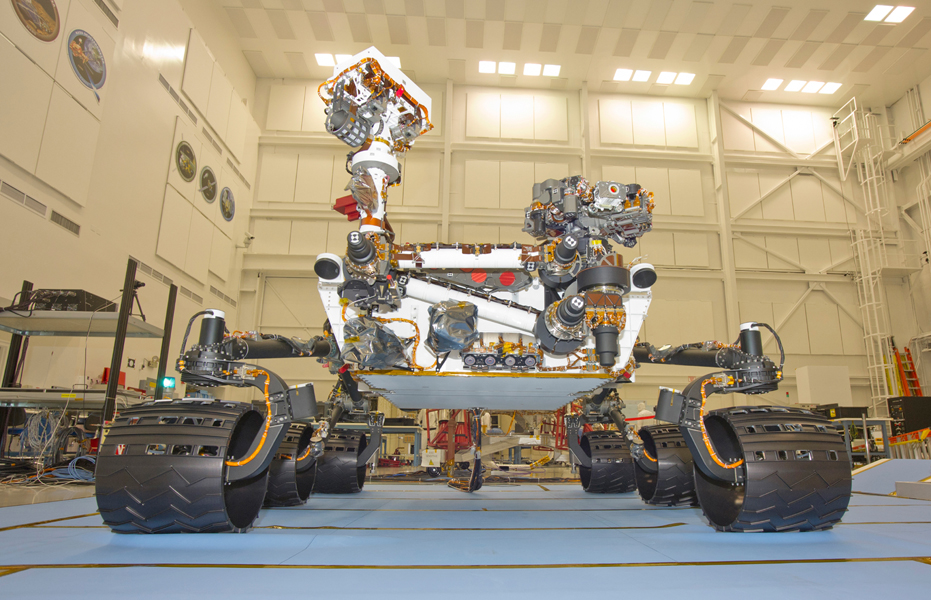
\includegraphics[scale=1.4]{images/img1-mars-rover}
	\caption{Front view of Mars Curiosity rover, Courtesy NASA/JPL-Caltech \cite{curiosity}}
	\label{fig:curiosity}
\end{figure}

The classification can be varied with new application areas and technologies. Although the specific applications are developed depending on the type and target task of the mobile robots, they share several cases to be handled such as sensor reading, tele-operation, to estimate the position and orientation, navigation and so on. These cases form the basics of a mobile robot application development. 

\section{Goal}
\label{sec:goal}
In this project, it is aimed to develop base applications using Robot Operating System (ROS) framework for the mobile robots of the type Autonomous Guided Vehicle (AGV) at Istanbul Technical University Robotics Laboratory named ITU-AGVs. The goal covers developing embedded software to be able to communicate with the microcontroller and developing on ROS framework for base tasks including simulation, sensor integration and reading, tele-operation, estimation of position and orientation, data collection and offline map building. It is aimed to provide these operations so that, they can be used as a basis –which ITU-AGVs lack– for developing specific applications. 


\section{Organization}
\label{sec:organization}
It is necessary to provide a background information in order to emphasize the project work. Hence in Chapter 2, information regarding Autonomous Guided Vehicles together with the details of ITU-AGVs are given and the kinematic model is derived. In Chapter 3, basics of Robot Operating System are provided with a brief review. Afterwards, all the work regarding the application development process is told in detailed in Chapter 4 and its subsections. Then, the overall outcomes, conclusions and possible future work are given in Chapter 5. 
% Some commands used in this file
%\newcommand{\package}{\emph}

\chapter{Autonomous Guided Vehicles \& ITU-AGVs}
\label{chap:agvs}

\begin{figure}[h]
	\centering
	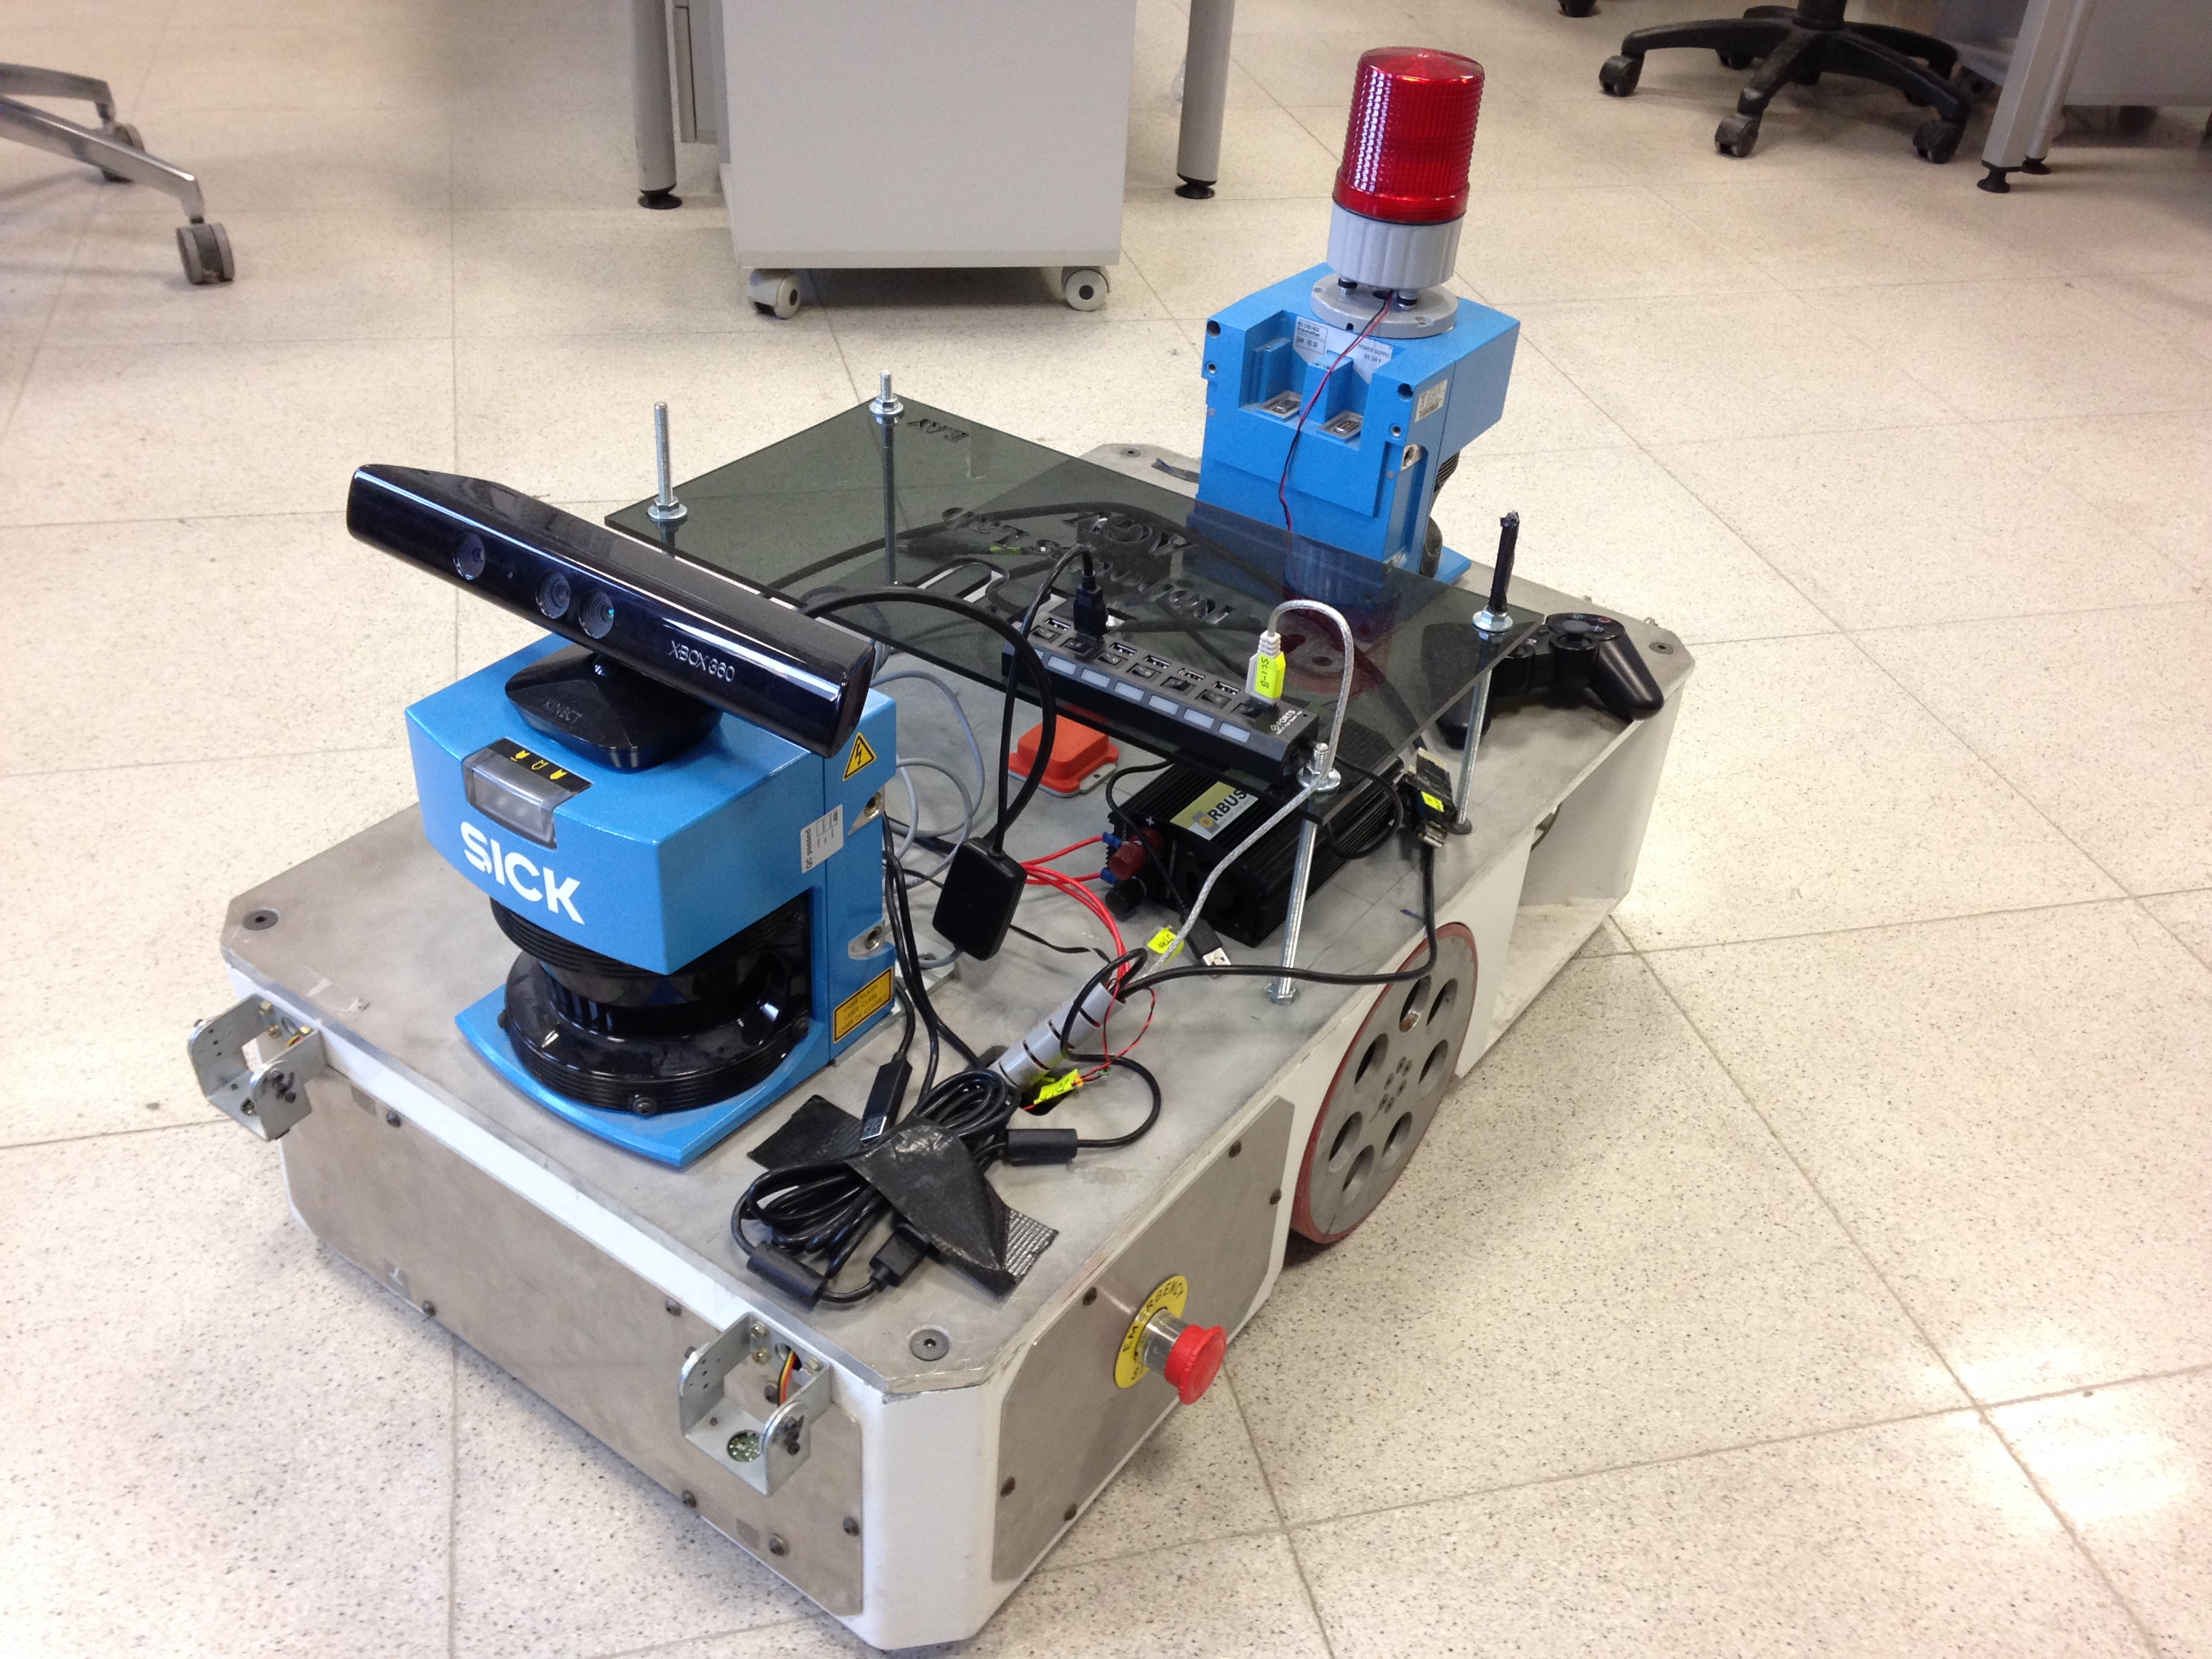
\includegraphics[scale=0.11]{images/agv1}
	\caption{One of the ITU-AGV robots}
	\label{fig:agv1}
\end{figure}

Autonomous Guided Vehicles (AGVs) or Automated Guided Vehicles are mobile robots that use lines or wires installed on the floor, cameras or laser sensors in order to navigate. They are industrial robots and their usual task is to carry objects or products in indoor or outdoor environments. Their market might be considered as the biggest one in mobile robotics \cite{alonzoKelly}. The present-day AGVs are mostly use laser sensors instead of floor wires or lines. 
\par
There are two identical AGVs that have built at Istanbul Technical University Robotics Laboratory named ITU-AGVs. Although they are designed as AGVs, they do not necessarily have to be used for warehouse automation or object carrying, but also they can be used as multi-purpose wheeled mobile robots. 

\section{Spesifications of ITU-AGVs}
\label{sec:specs of agvs}
ITU-AGV robots are differential-driven, bidirectional mobile robots with two driving wheels and two caster wheels (Figure ~\ref{fig:agv1}). They have two 250 Watt Maxon EC54 brushless DC motors with a ratio of 1:100 reduction gear-boxes. The motors are driven by using Maxon EPOS 70/10 drivers. The robots are powered with two serially connected batteries with 12 V output voltage and 26 Ah charge, each. To supply motors and all other hardware, there are 5 V, 12 V and 24 V voltage regulators in order to acquire necessary voltage levels. 
\par
ITU-AGVs have 49 cm width, 82 cm length and 22 cm height. The driving wheels have 10 cm radius. They weight approximately 70 kg without the additional sensors and their payload is approximately 100 kg for each. 
\par
It is possible to install various sensors on the robot. To make it a multi-purpose robot that can be used in different future projects, two laser range finder sensors, a Microsoft Kinect sensor, an inertial measurement unit (IMU) and four analog distance sensors are mounted on ITU-AGVs. The microcontrollers provided for ITU-AGVs were Texas Instruments TMS320F28335 with Spectrum Digital eZdsp F28335 board. 
The power chart of ITU-AGVs can be seen in Figure ~\ref{fig:agvPower}.

\begin{figure}
	\centering
	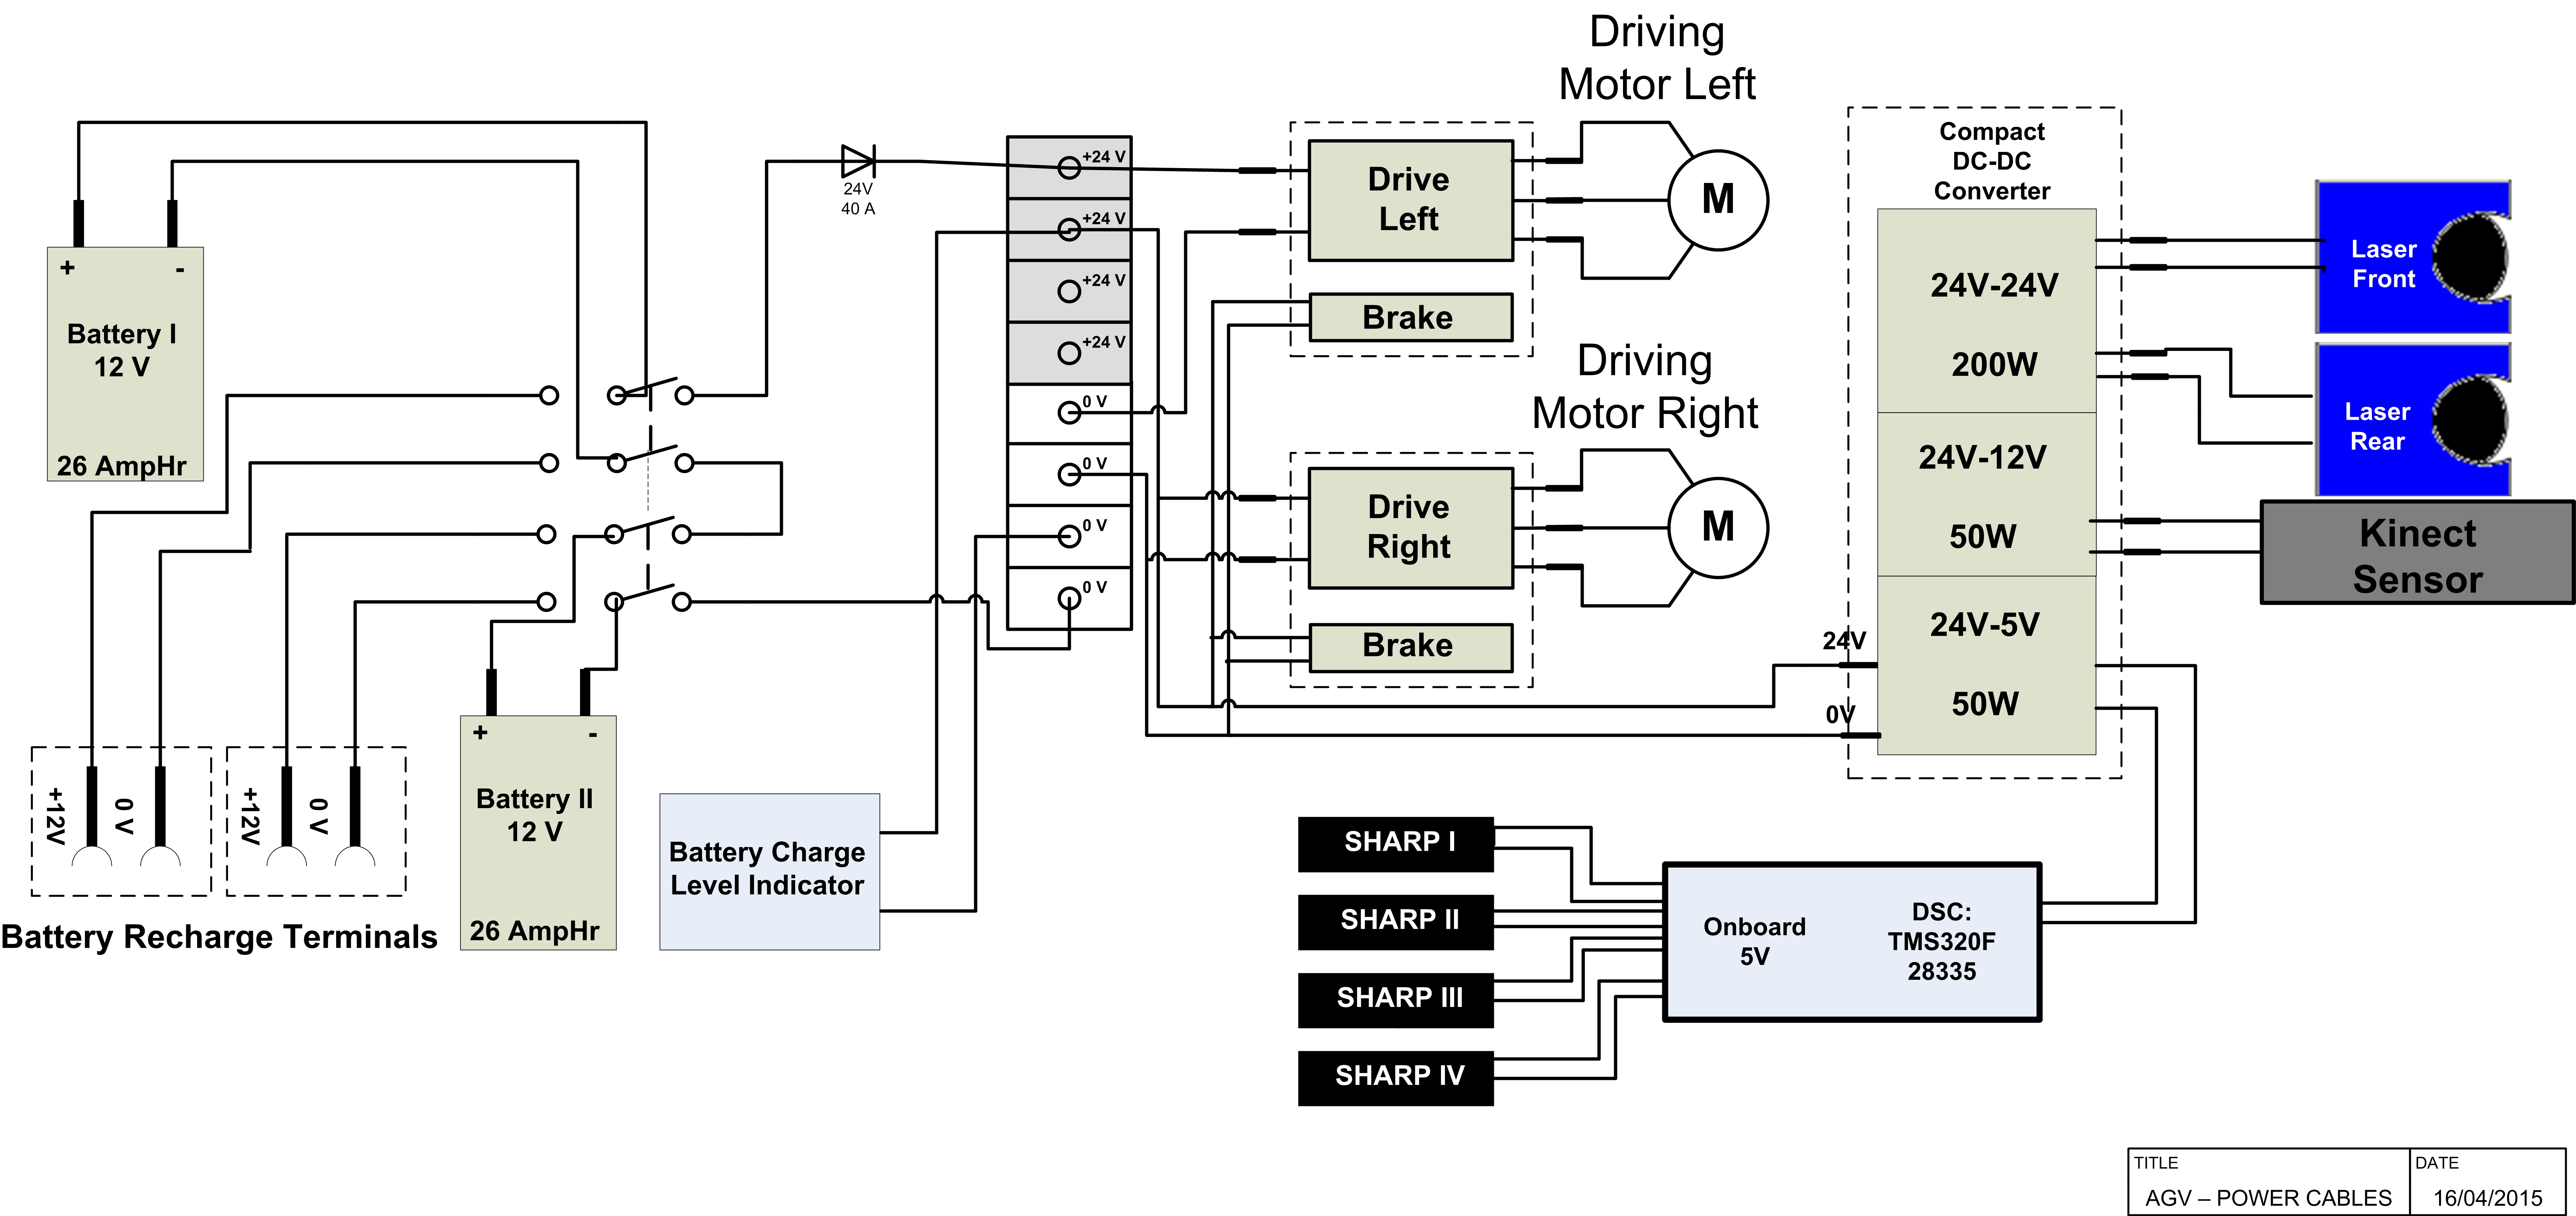
\includegraphics[scale=0.42]{images/img2-agvPower}
	\caption{Power chart of ITU-AGVs}
	\label{fig:agvPower}
\end{figure}

\section{Sensors and Low Level Processing Layer (LLPL)}
\label{sec:sensors and llpl}

\subsection{Light Detection and Ranging (LIDAR) Sensors}
\label{subsec:lidar}
There are two light detection and ranging (LIDAR) sensors mounted on ITU-AGVs. These are SICK Laser Measurement System LMS200 (Figure ~\ref{fig:kinect-sick}) and they are indoor sensors with 180 degrees scanning field and 10 meters range. Their working principle is based on time of flight measurement of reflected infrared light beam emitted by the sensor. In order to have a radial range, a rotating mirror deflects the emitted infrared light to the environment. The sensor outputs the distance values in the range for 180 degrees at 9600 baud rate ~\cite{sickDatasheet}.

\subsection{Inertial Measurement Unit (IMU)}
\label{subsec:imu}
Using an internal measurement unit is useful for position and orientation estimation. Hence, a 3 DOF Xsens MTi Attitude and Heading Reference System (AHRS) is mounted on ITU-AGVs (Figure ~\ref{fig:xsens}). Xsens MTi is an IMU that has magnetometers, accelerometers and gyroscopes and it outputs orientation, acceleration, rate of turn and earth magnetic data in three dimensions ~\cite{xsensDatasheet}. It has small dimensions ($58\times58\times22$ mm) and low weight (50 g). The sensor is mounted along the center of the robot. 

\subsection{Infrared Distance Sensors}
\label{subsec:infrared sensors}
Four infrared distance sensors are mounted on front and rear of ITU-AGVs in order to understand if there is a hole or a stair while the robots are moving in the environment. The infrared distance sensors are analog Sharp sensors with 30 cm ranges. 

\subsection{Microsoft Kinect Sensor}
\label{subsec:kinect}
Microsoft Kinect sensor has an RGB camera with $1280\times960$ resolution, an infrared emitter and infrared depth sensor to get the depth information by measuring the distance of objects from the reflected infrared beams that have emitted by the sensor, a microphone array, an accelerometer and a tilt motor ~\cite{kinectSpecs}. It is mounted on the front of ITU-AGVs (Figure ~\ref{fig:kinect-sick}) and its RGBD output can be used for many applications. 

\begin{figure}[h]
	\centering
	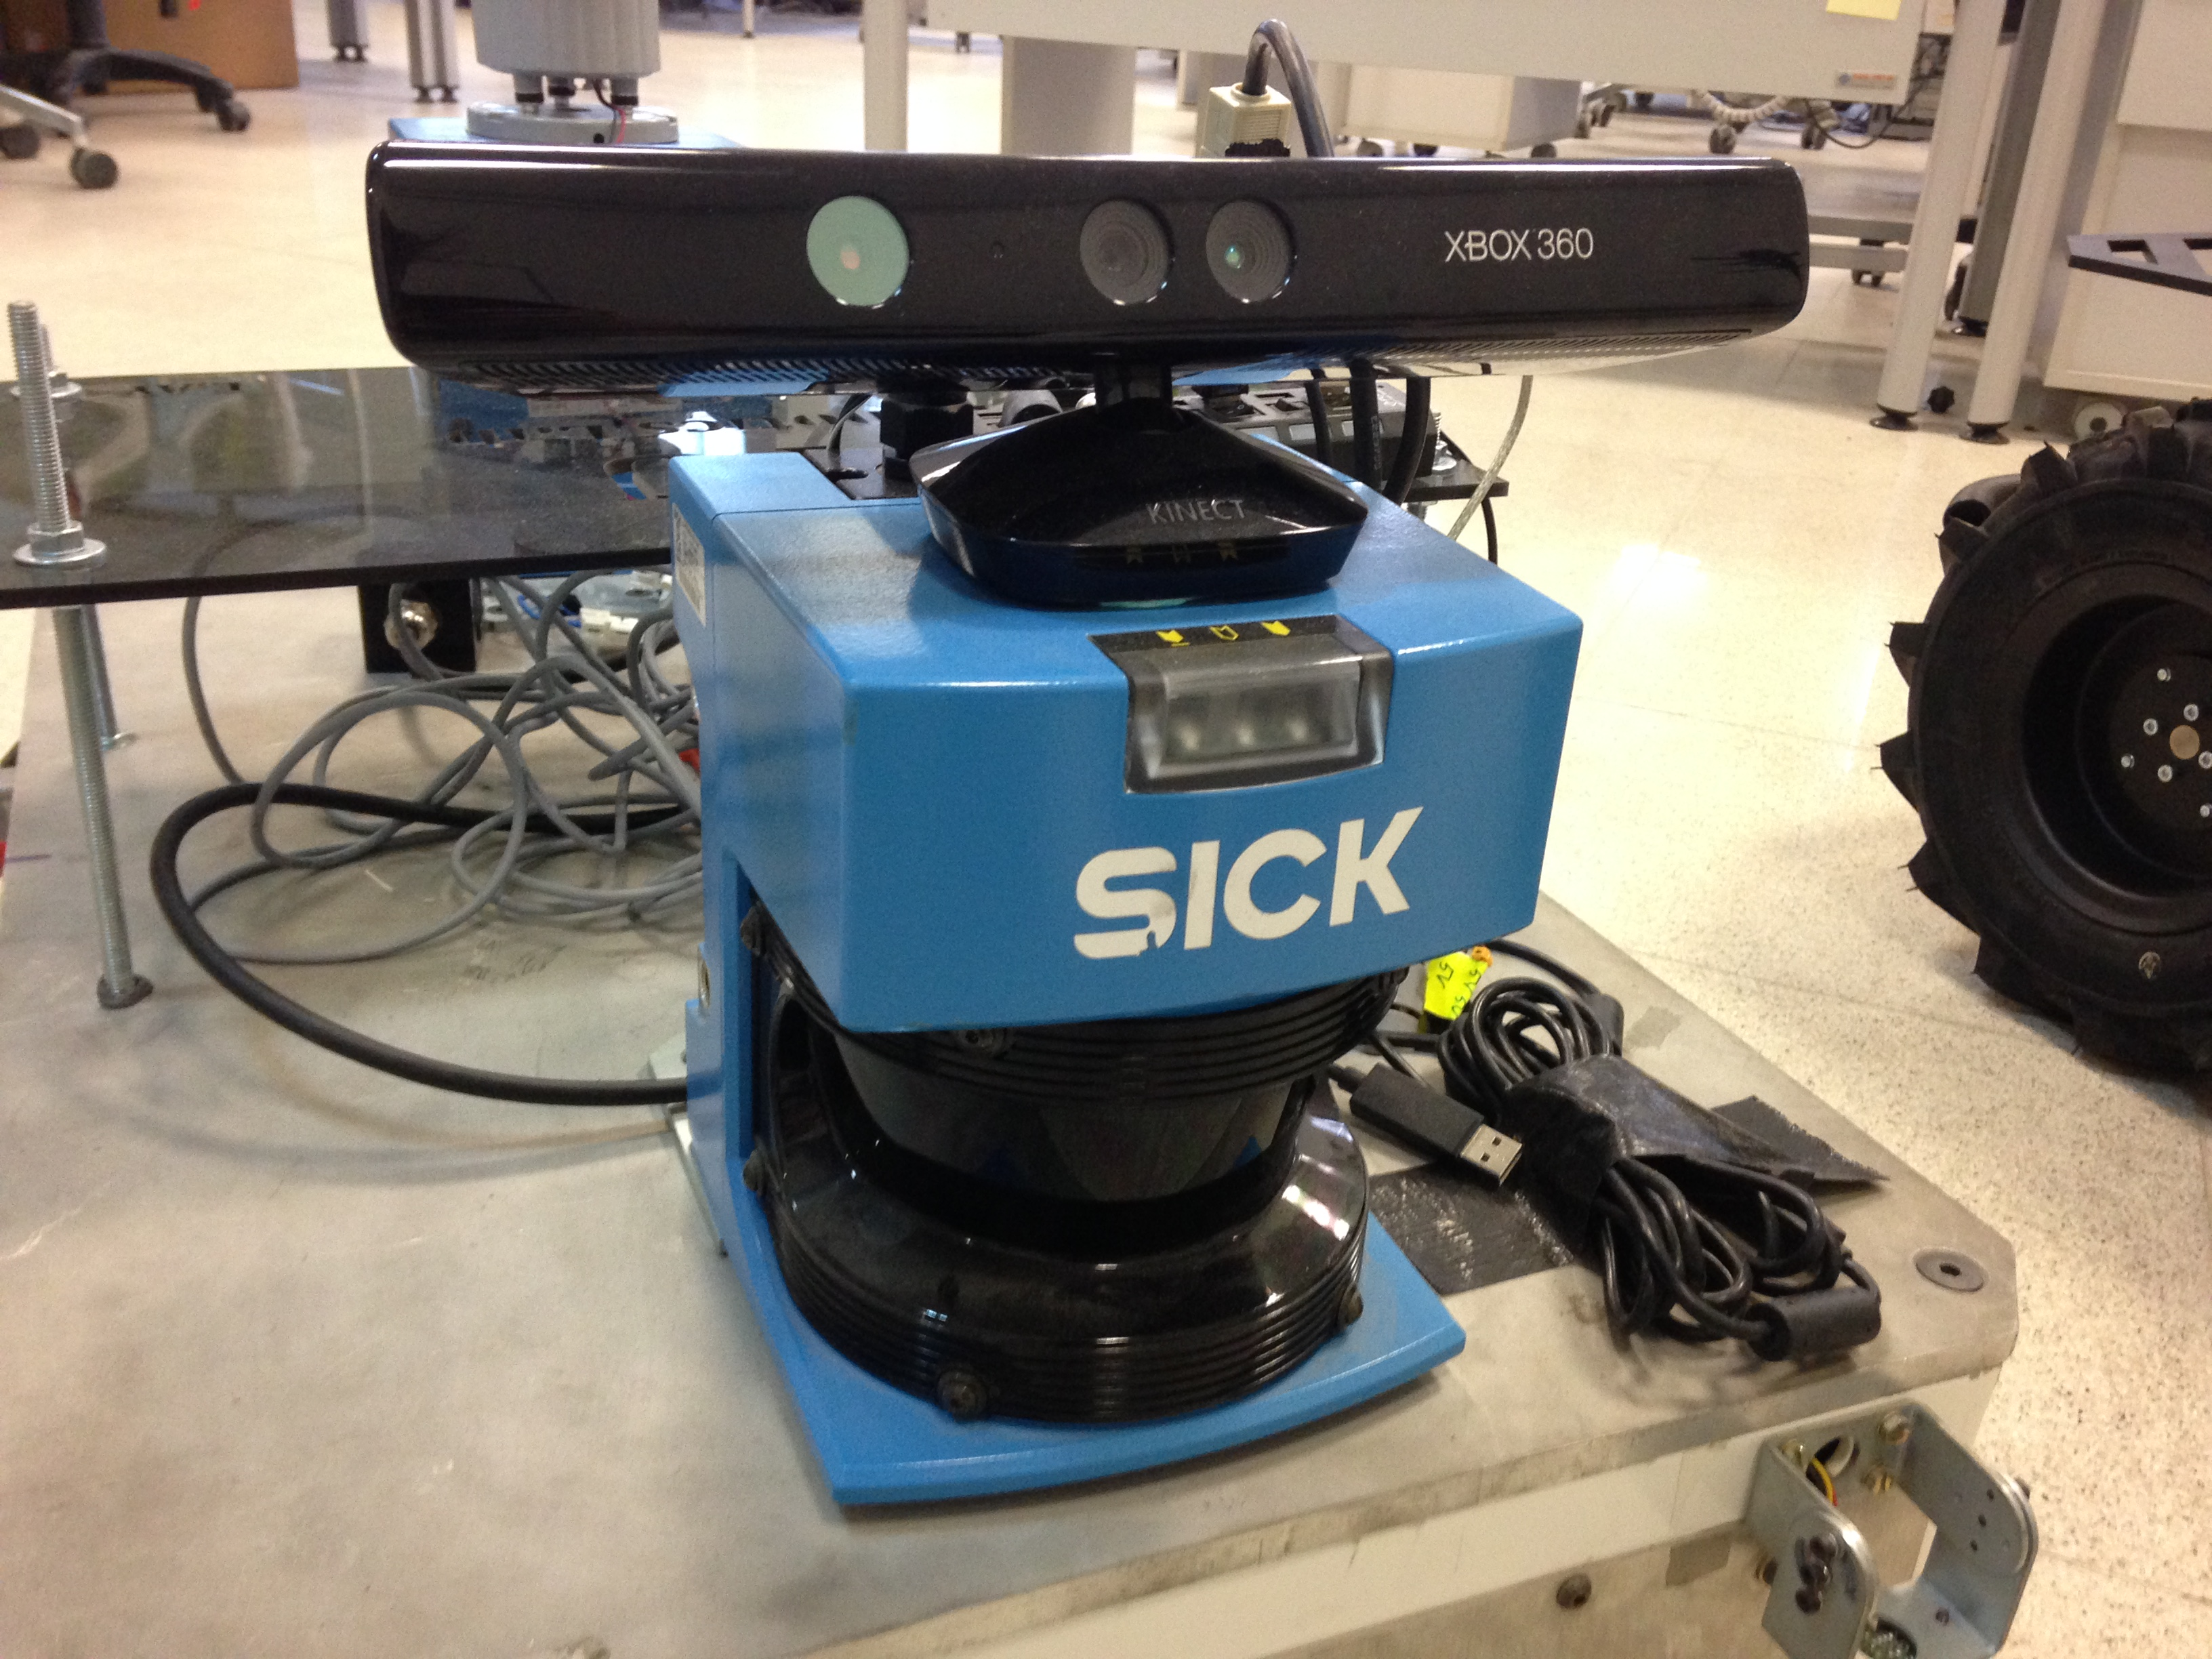
\includegraphics[scale=0.1]{images/kinect-sick}
	\caption{Microsoft Kinect and Sick LMS200 sensors on ITU-AGVs}
	\label{fig:kinect-sick}
\end{figure}

\subsection{Motor Encoders}
\label{subsec:encoder}
Motor encoders are also vital for estimation of position and orientation. The motors have three channels, 500 counts per turn HEDL 9140 encoders.

\begin{figure}
	\centering
	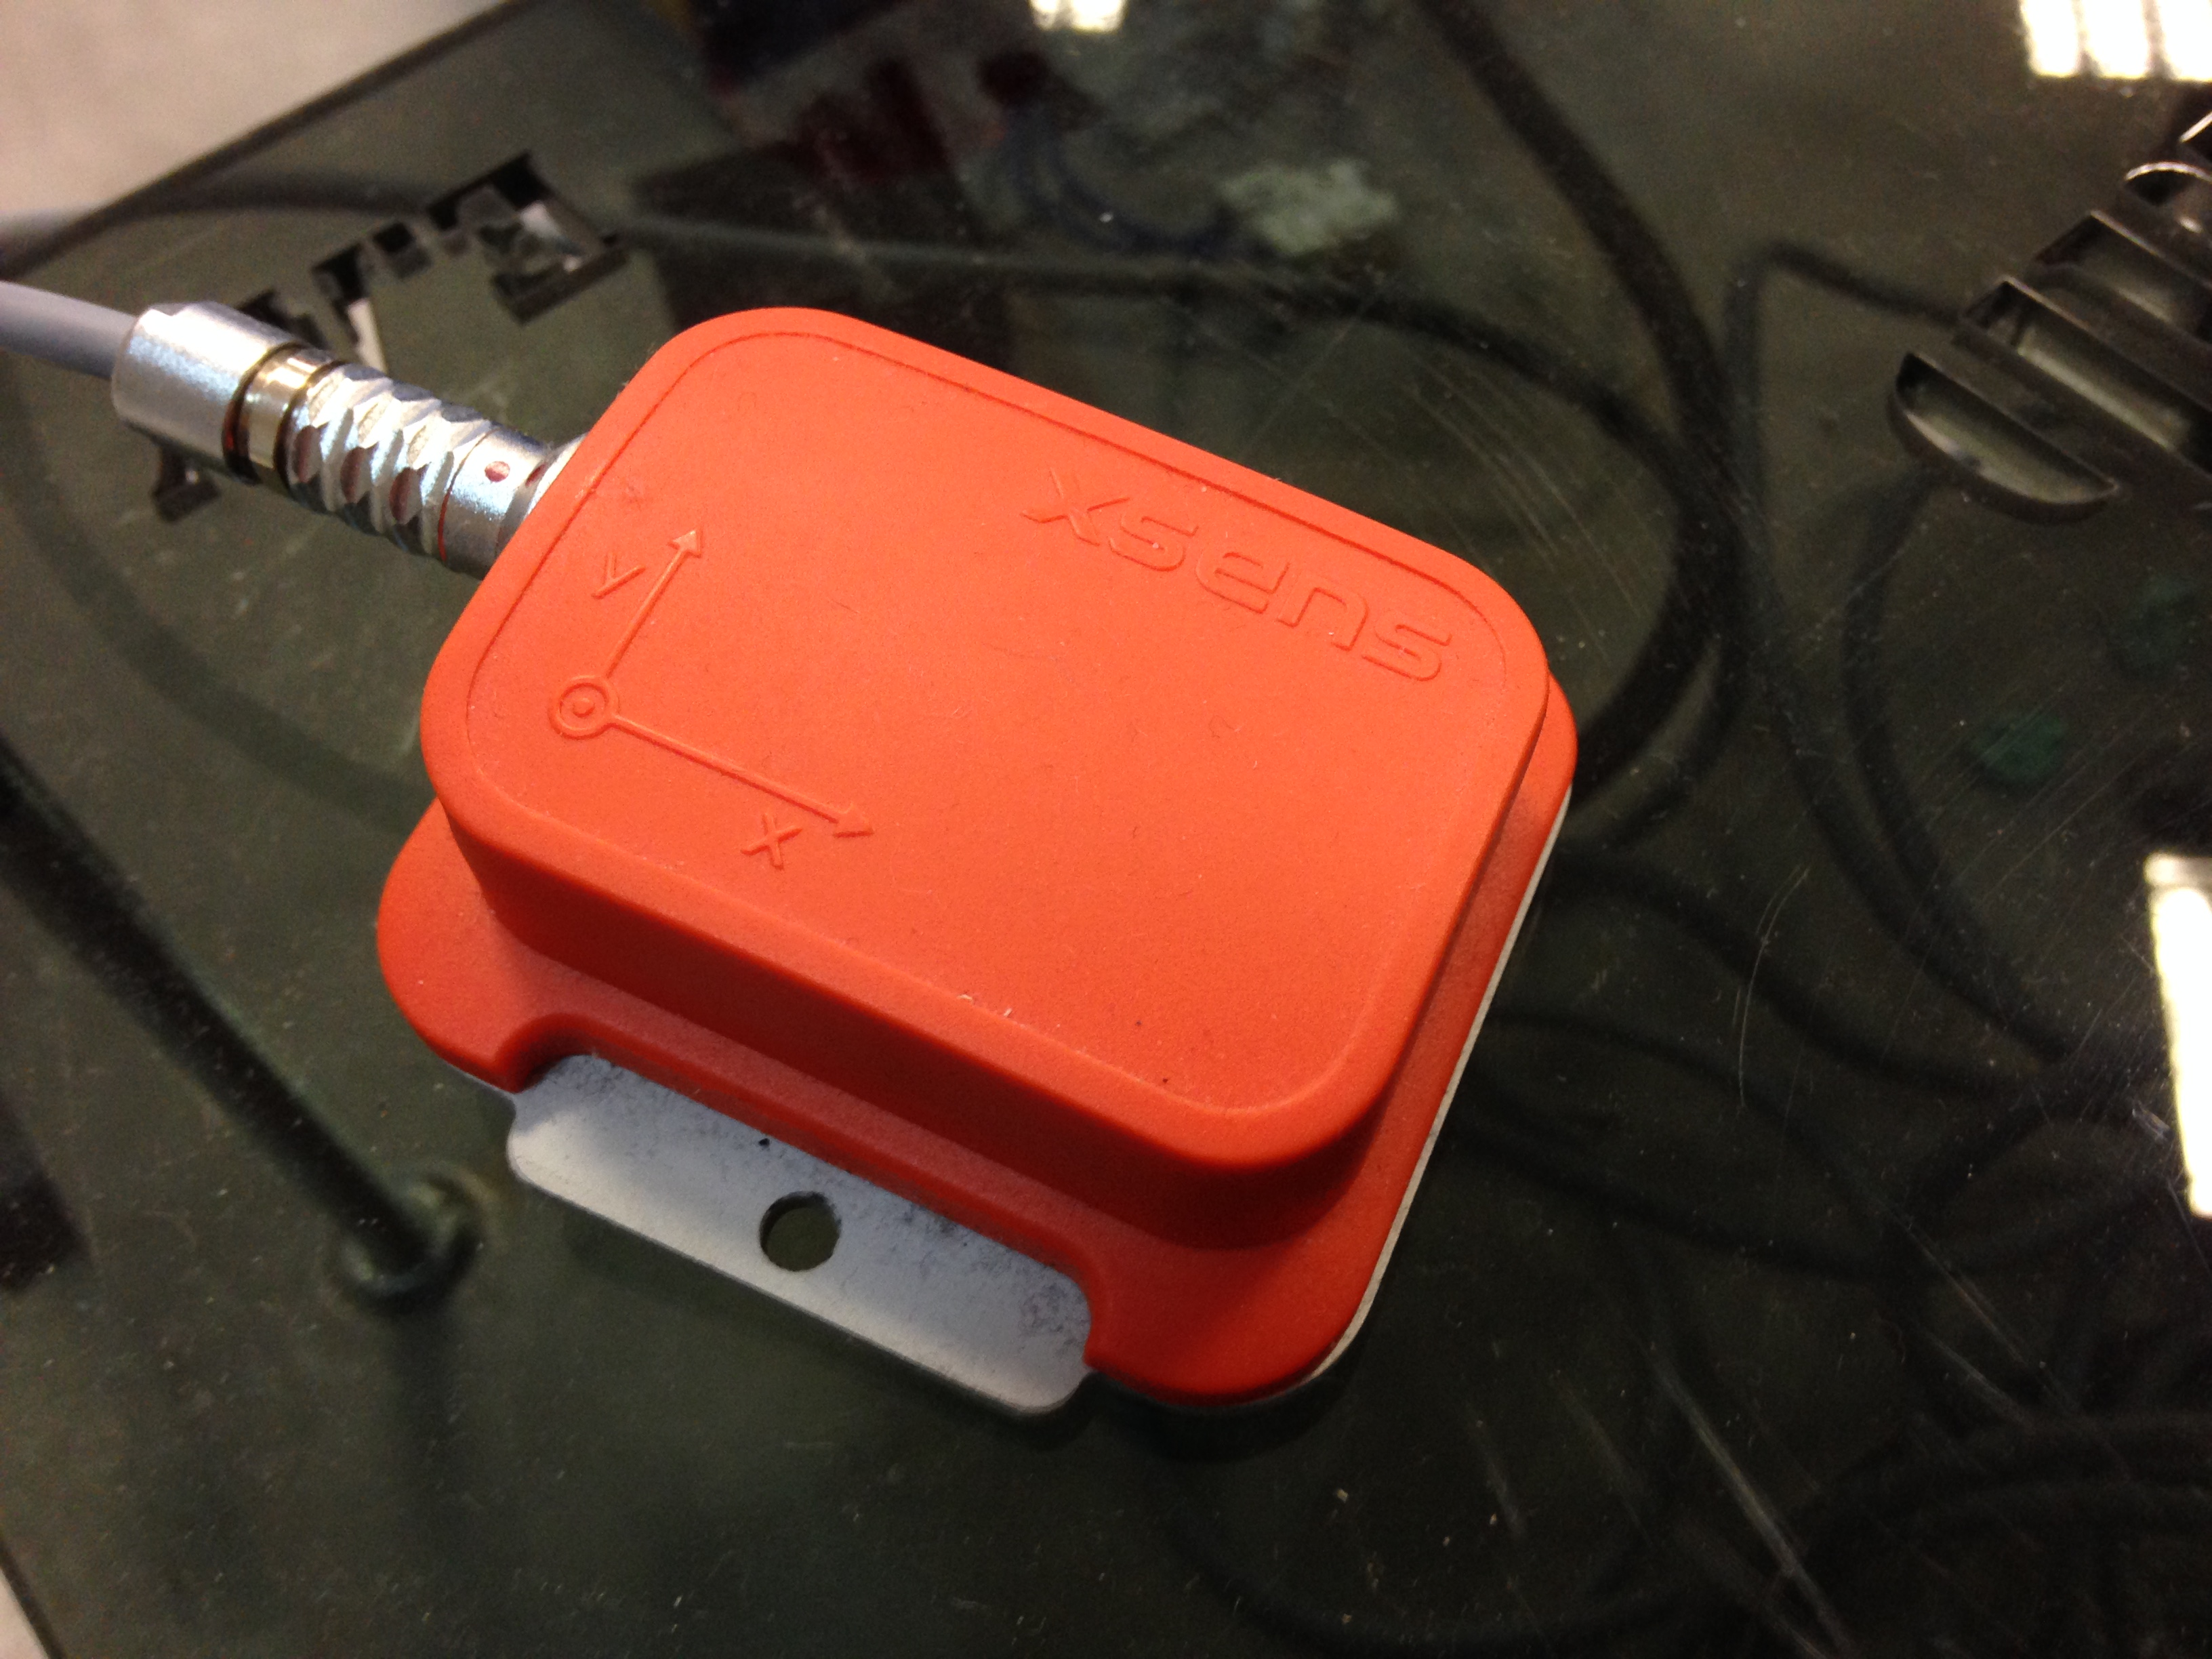
\includegraphics[scale=0.1]{images/xsens}
	\caption{Xsens MTi sensor on ITU-AGVs}
	\label{fig:xsens}
\end{figure}


\subsection{Low Level Processing Layer (LLPL)}
\label{subsec:llpl}
As in many robotic systems, there are two processing layers in ITU-AGVs. Low Level Processing Layer (LLPL) is responsible of getting commands from High Level Processing Layer (HLPL), communicating with motor drivers and sending necessary signals to drive the motors, requesting the encoder values and send them to HLPL. In addition to these flow, the analog distance sensors are also connected to LLPL. The microcontrollers used at LLPL on ITU-AGVs are Texas Instruments TMS320F28335 with Spectrum Digital eZdsp F28335 board. 
\par
The eZdsp F28335 is a stand-alone board with TMS320F28335 Digital Signal Controller. It works at 150 Mhz operating speed and it has 32-bit floating point unit, 68 KB RAM, 512 KB Flash memory, 256 KB off-chip SRAM memory, 12-bit Analog to Digital Converter (ADC), 30 MHz input clock, RS232 and CAN connectors, USB JTAG controller and multiple General Purpose Input Output (GPIO) pins~\cite{ezdspDatasheet}.


\section{Kinematics}
\label{sec:kinematics}
\begin{figure}
	\centering
	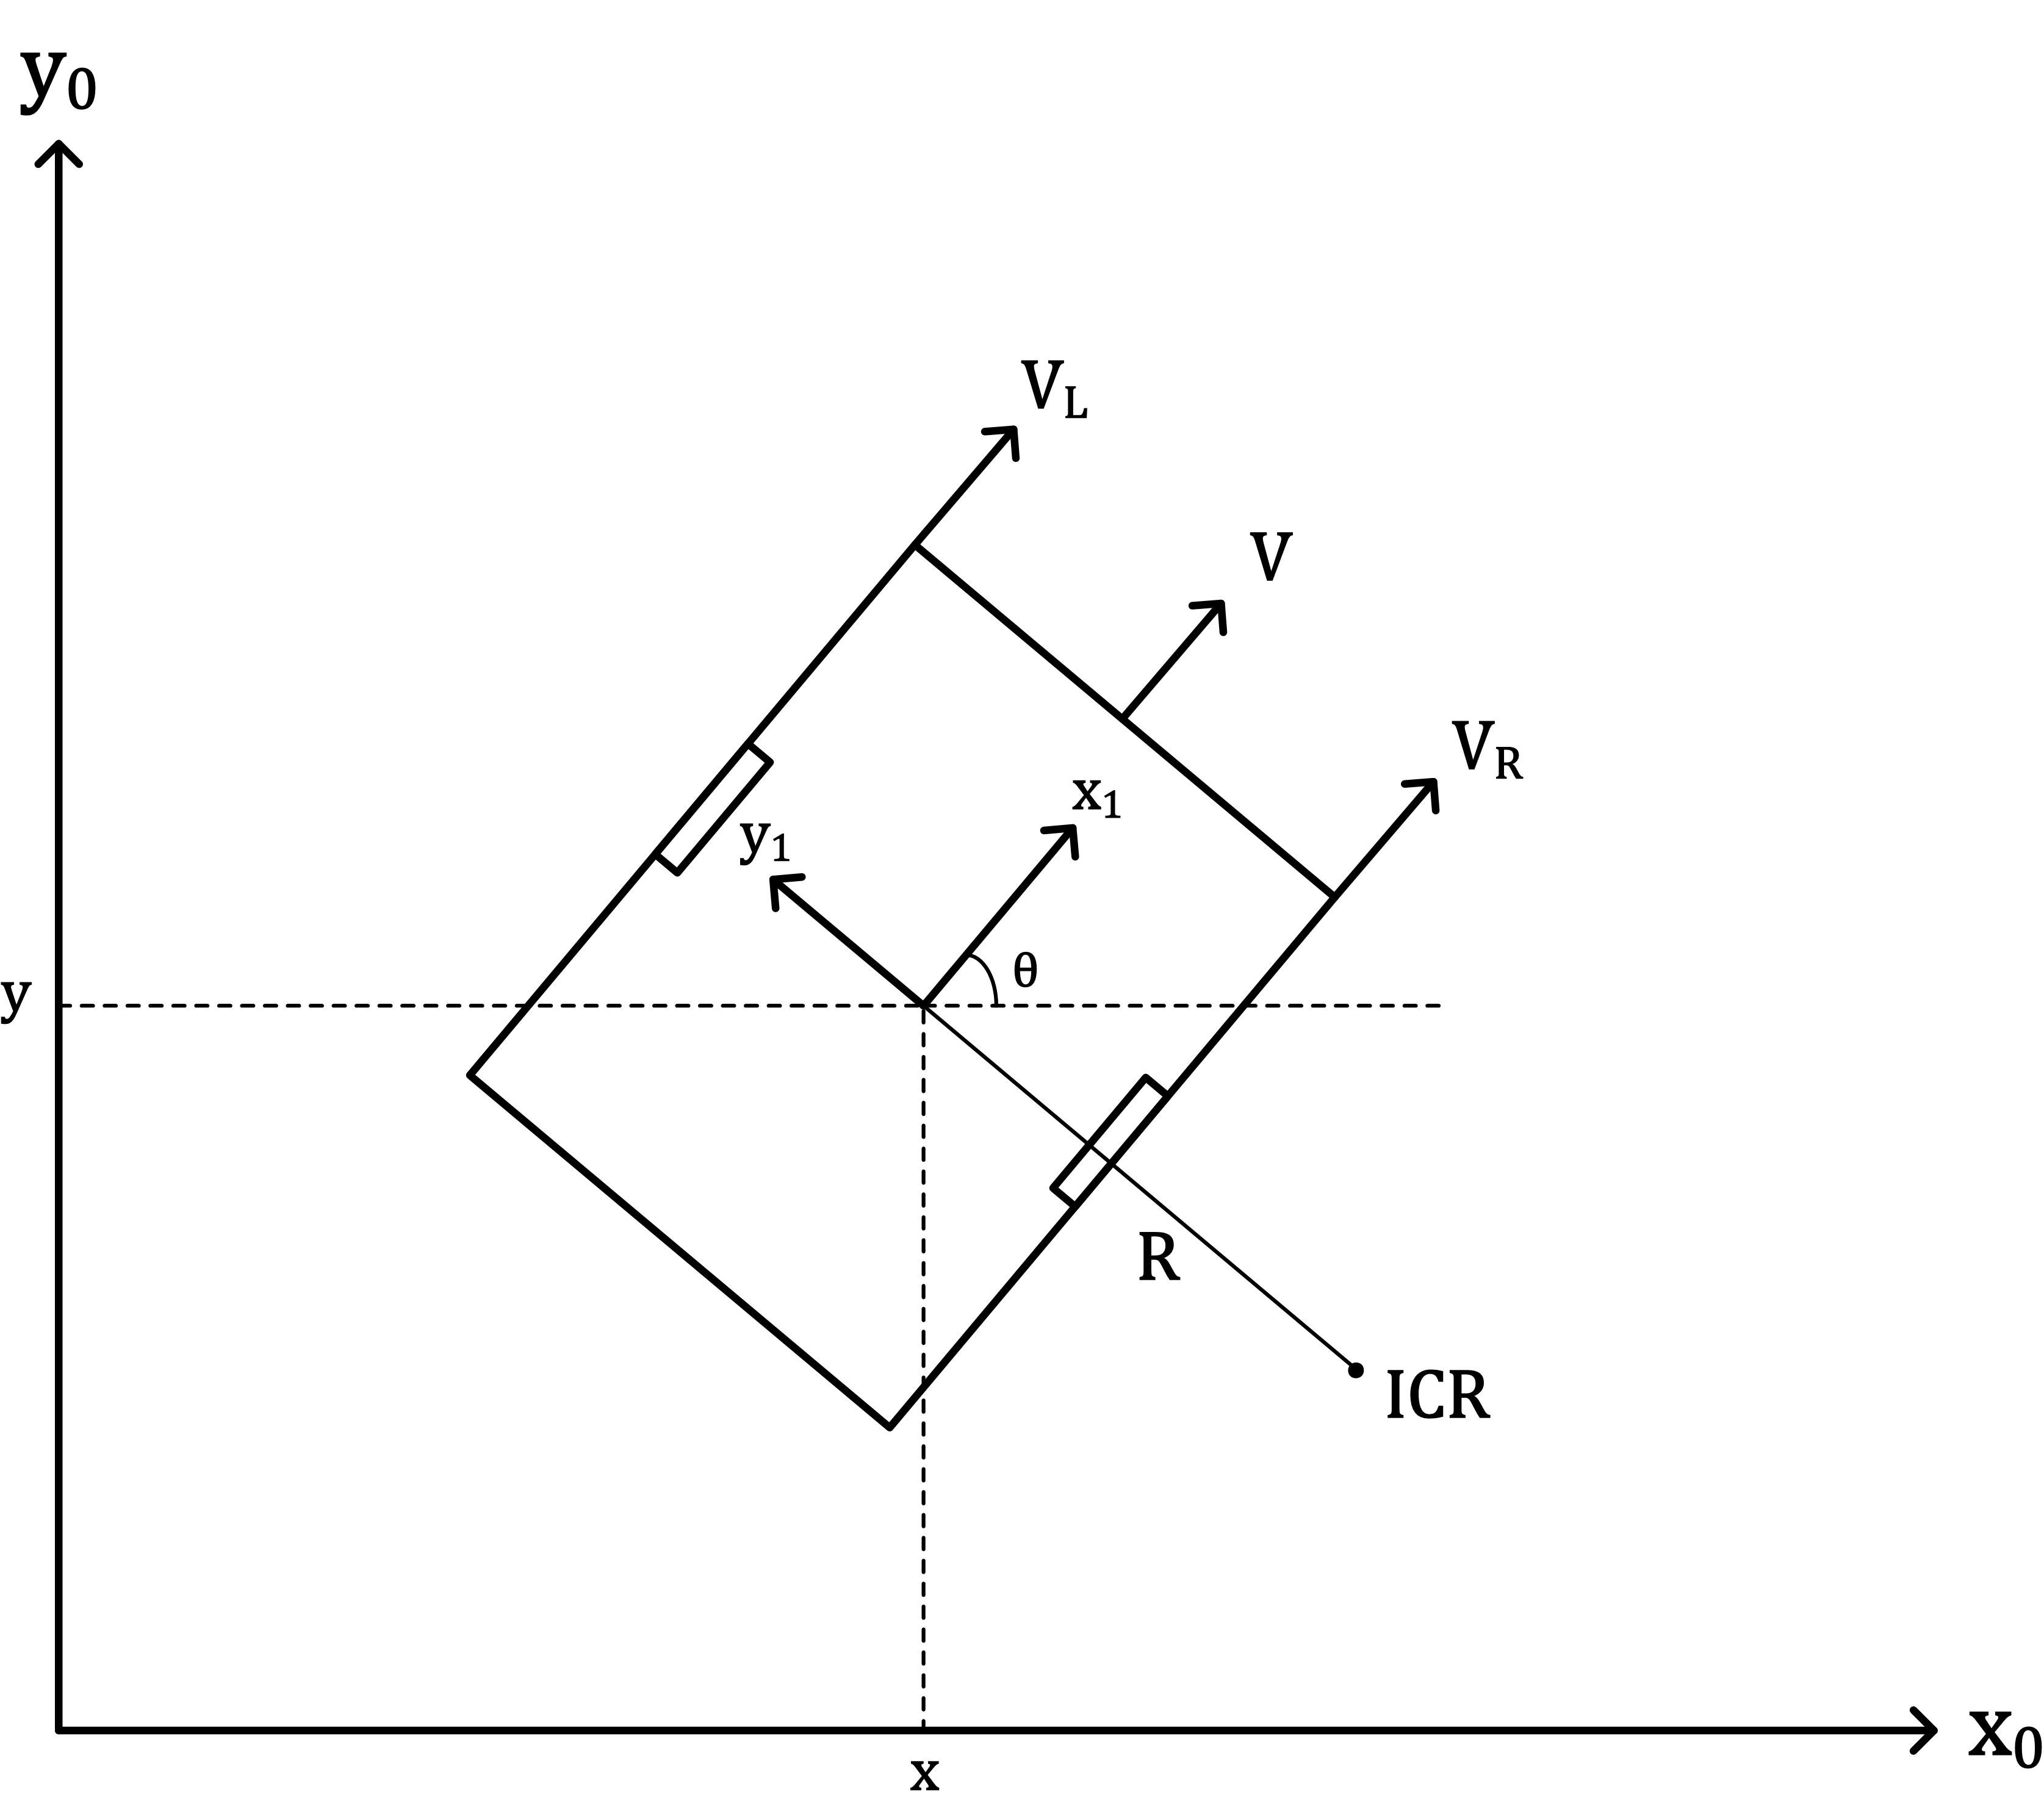
\includegraphics[scale=0.9]{images/kinematics_fig}
	\caption{Frames of a mobile robot in 2D}
	\label{fig:kinematics}
\end{figure}

It is necessary to construct the kinematic model of ITU-AGVs since it will be used in application development. Consider \textit{r} as the radius of the wheels, \textit{R} as the radius of rotation, \textit{L} as the length between the wheels, $\omega$(\textit{t}) and \textit{V}(\textit{t}) as the angular and linear velocities of the robot, \textit{V\textsubscript{L}}(\textit{t}) and $\omega$\textit{\textsubscript{L}}(\textit{t}) as the linear and angular velocities of the left wheel, \textit{V\textsubscript{R}}(\textit{t}) and $\omega$\textit{\textsubscript{L}}(\textit{t}) as the linear and angular velocities of the right wheel, $\theta$ is the angle between x axis of the frames, \textit{x\textsubscript{0}} and \textit{y\textsubscript{0}} as the coordinate axis of the world frame and \textit{x\textsubscript{1}} and \textit{y\textsubscript{1}} as the coordinate axis of the robot frame as in Figure~\ref{fig:kinematics}. 
\par
At any time instant \textit{t}, the linear velocities at left and right wheels can be calculated from the product of their angular velocities and radius;
\par 
\begin{equation}
\textit{V\textsubscript{L}}(\textit{t}) = \omega\textit{\textsubscript{L}}(\textit{t})\cdot\textit{r}
\end{equation}

\begin{equation}
\textit{V\textsubscript{R}}(\textit{t}) = \omega\textit{\textsubscript{R}}(\textit{t})\cdot\textit{r}
\end{equation}

The linear velocities also can be written from the angular velocity of the robot;
\begin{equation}
\textit{V\textsubscript{L}}(\textit{t}) = \omega(\textit{t})\cdot(\textit{R}-\frac{L}{2})
\end{equation}

\begin{equation}
\textit{V\textsubscript{R}}(\textit{t}) = \omega(\textit{t})\cdot(\textit{R}+\frac{L}{2})
\end{equation}

So, combining and solving these equations yields the angular velocity of the robot;
\begin{equation}
\omega(\textit{t}) = \frac{\textit{V\textsubscript{R}}(\textit{t})-\textit{V\textsubscript{L}}(\textit{t})}{L}
\end{equation}

The linear velocity of the robot is simply;
\begin{equation}
\textit{V}(\textit{t}) = \frac{\textit{V\textsubscript{R}}(\textit{t})+\textit{V\textsubscript{L}}(\textit{t})}{2}
\end{equation}

The kinematic model in the world frame can be constructed as;
\begin{equation}
\begin{bmatrix}
\textit{v}_{x\textsubscript{0}}(\textit{t})\\
\textit{v}_{y\textsubscript{0}}(\textit{t})\\
\dot{\theta}(\textit{t})
\end{bmatrix}=
\begin{bmatrix}
cos\theta & 0\\
sin\theta & 0\\
0         & 1
\end{bmatrix}\cdot
\begin{bmatrix}
\textit{V}(\textit{t})\\
\omega(\textit{t})\\
\end{bmatrix}
\end{equation} 

and the kinematic model in the robot frame can be constructed as;
\begin{equation}
\begin{bmatrix}
\textit{v}_{x\textsubscript{1}}(\textit{t})\\
\textit{v}_{y\textsubscript{1}}(\textit{t})\\
\dot{\theta}(\textit{t})
\end{bmatrix}=
\begin{bmatrix}
\frac{r}{2}  & \frac{r}{2}\\
0            & 0\\
-\frac{R}{L} & \frac{R}{L}
\end{bmatrix}\cdot
\begin{bmatrix}
\omega_{L}(\textit{t})\\
\omega_{R}(\textit{t})\\
\end{bmatrix}
\end{equation} 
where $\textit{v}_{x\textsubscript{0}}(\textit{t}),\textit{v}_{y\textsubscript{0}}(\textit{t}),\textit{v}_{x\textsubscript{1}}(\textit{t})$ and $\textit{v}_{y\textsubscript{1}}(\textit{t})$ are the velocities at frame axis $x_{0}, y_{0}, x_{1}$ and $y_{1}$.
% Some commands used in this file
%\newcommand{\package}{\emph}

\chapter{Robot Operating System (ROS)}
\label{chap:ros}

\section{Fundamentals of ROS}
\label{sec:fundamentals of ros}
Robot Operating System (ROS) framework has shown an increasing popularity at robotics applications since it was first released at 2009 by Willow Garage. Even though it has “operating system” in its name, ROS is not an actual operating system. It might be classified as a \textit{framework} or a \textit{middleware} that serves various useful tools. 
\par
The hardware on the present-day robots differs broadly. To prevent writing codes again for same or similar tasks on robots with different hardware, or in others words to avoid reinventing the steel, by providing an environment is the basic logic behind the ROS. 
\par
ROS is designed to be peer-to-peer, tool based, multi-lingual, thin, free and open-source ~\cite{Quigley09}. Every ROS application consists of computational units or programs named \textit{nodes} and communications and relationships of them. The \textit{nodes} can communicate over \textit{topics} by passing certain data named \textit{messages}. 
\par
ROS is based on four fundamentals; passing messages by publishing or subscribing to topics, passing messages using services, recording messages and playing-back when necessary and having a dynamically reconfigurable distributed parameter server ~\cite{rosCoreComponents}. Using these core features, it is possible to perform many simple and complex tasks. 

\section{A Brief Review of ROS}
\label{sec:brief review of ros}
ROS project officially supports Ubuntu and pre-compiled ROS distributions are supplied officially. However, since it is an open-source project, its source files are available and it is possible to compile them on similar platforms. Hence there are experimental pre-compiled repositories available such as the one for the Raspbian operating system of Raspberry Pi development boards ~\cite{rosRaspbian}.
\par
ROS file system is based on unit software organizations called \textit{packages} and organization of related packages called \textit{metapackages} ~\cite{rosFileSystem}. There used be \textit{stack} organization but they have replaced with \textit{metapackages} in the newer ROS distributions. Every package can contain libraries, executables, source codes, launch files, scripts and so on. 
\par
ROS uses a build system called \textit{catkin} which combines CMake build system with Python codes. A build system is the system that constitutes target files which might be executables, libraries, header files from the source code ~\cite{rosCatkin}. ROS changed its build system to \textit{catkin} on and after the Groovy distribution. 
\par
As mentioned in the previous section, one of the design goals of ROS was to be multi-lingual. ROS supports C++ and Python. So the nodes can be written in both C++ and Python and a node that has written in C++ can communicate with the one that has written in Python and vice versa. 
\par
ROS does not only provide features to make the nodes communicate in certain methods, but it also provides several tools to make diagnostics and debug. For example, there are tools to see the nodes and topics as a graph, to plot messages according to time or to find out the message passing frequency on a topic. Also there are simulation and visualization environments working with ROS such as Rviz and Gazebo. 
\par
ROS framework forms an environment for reuse the codes. There are many message type definitions for common messages and also it is easy to create custom messages. Many sensors and hardware have their ROS libraries and drivers which makes easier and faster to install various hardware. Finally, ROS has an involved and wide community. All these features make ROS preferable and usable. 


% Some commands used in this file
%\newcommand{\package}{\emph}

\chapter{Mobile Robot Application Development}
\label{chap:app dev}
It is needed to have a software basis for ITU-AGVs that will be used to develop specific applications for various tasks in the future possible projects, theses and works. ITU-AGVs have built before ROS was developed. At the time when ITU-AGVs built, the software systems that used were different and custom so the software of the robots was written concerning them which became out-of-date now.
\par 
As mentioned previously in the Introduction chapter, the goal is to construct a set of applications for the basic problems and needs using up-to-date tools. It is desired to write the embedded code for LLPL so the robots can be communicate with ROS and to develop ROS applications for tele-operation, sensor integration and reading, odometry estimation, data collection and offline map building. With realization of this basis, ITU-AGVs can be used as multi-purpose indoor land vehicle kits available using rapidly for educational purposes, theses, autonomous system design and algorithm development at ITU Robotics Laboratory.
\par
The processing work is divided with a hierarchy. Low Level Processing Layer (LLPL) is responsible for getting commands, communicating motor drivers to drive the motors as desired in the given commands, requesting encoder values and sending them to High Level Processing Layer. High Level Processing Layer is responsible for complex calculations and is the part where the ROS runs. The signal chart of ITU-AGVs can be seen in Figure ~\ref{fig:agvSignal}. The project is started with LLPL work and then HLPL after. 

\begin{figure}[h]
	\centering
	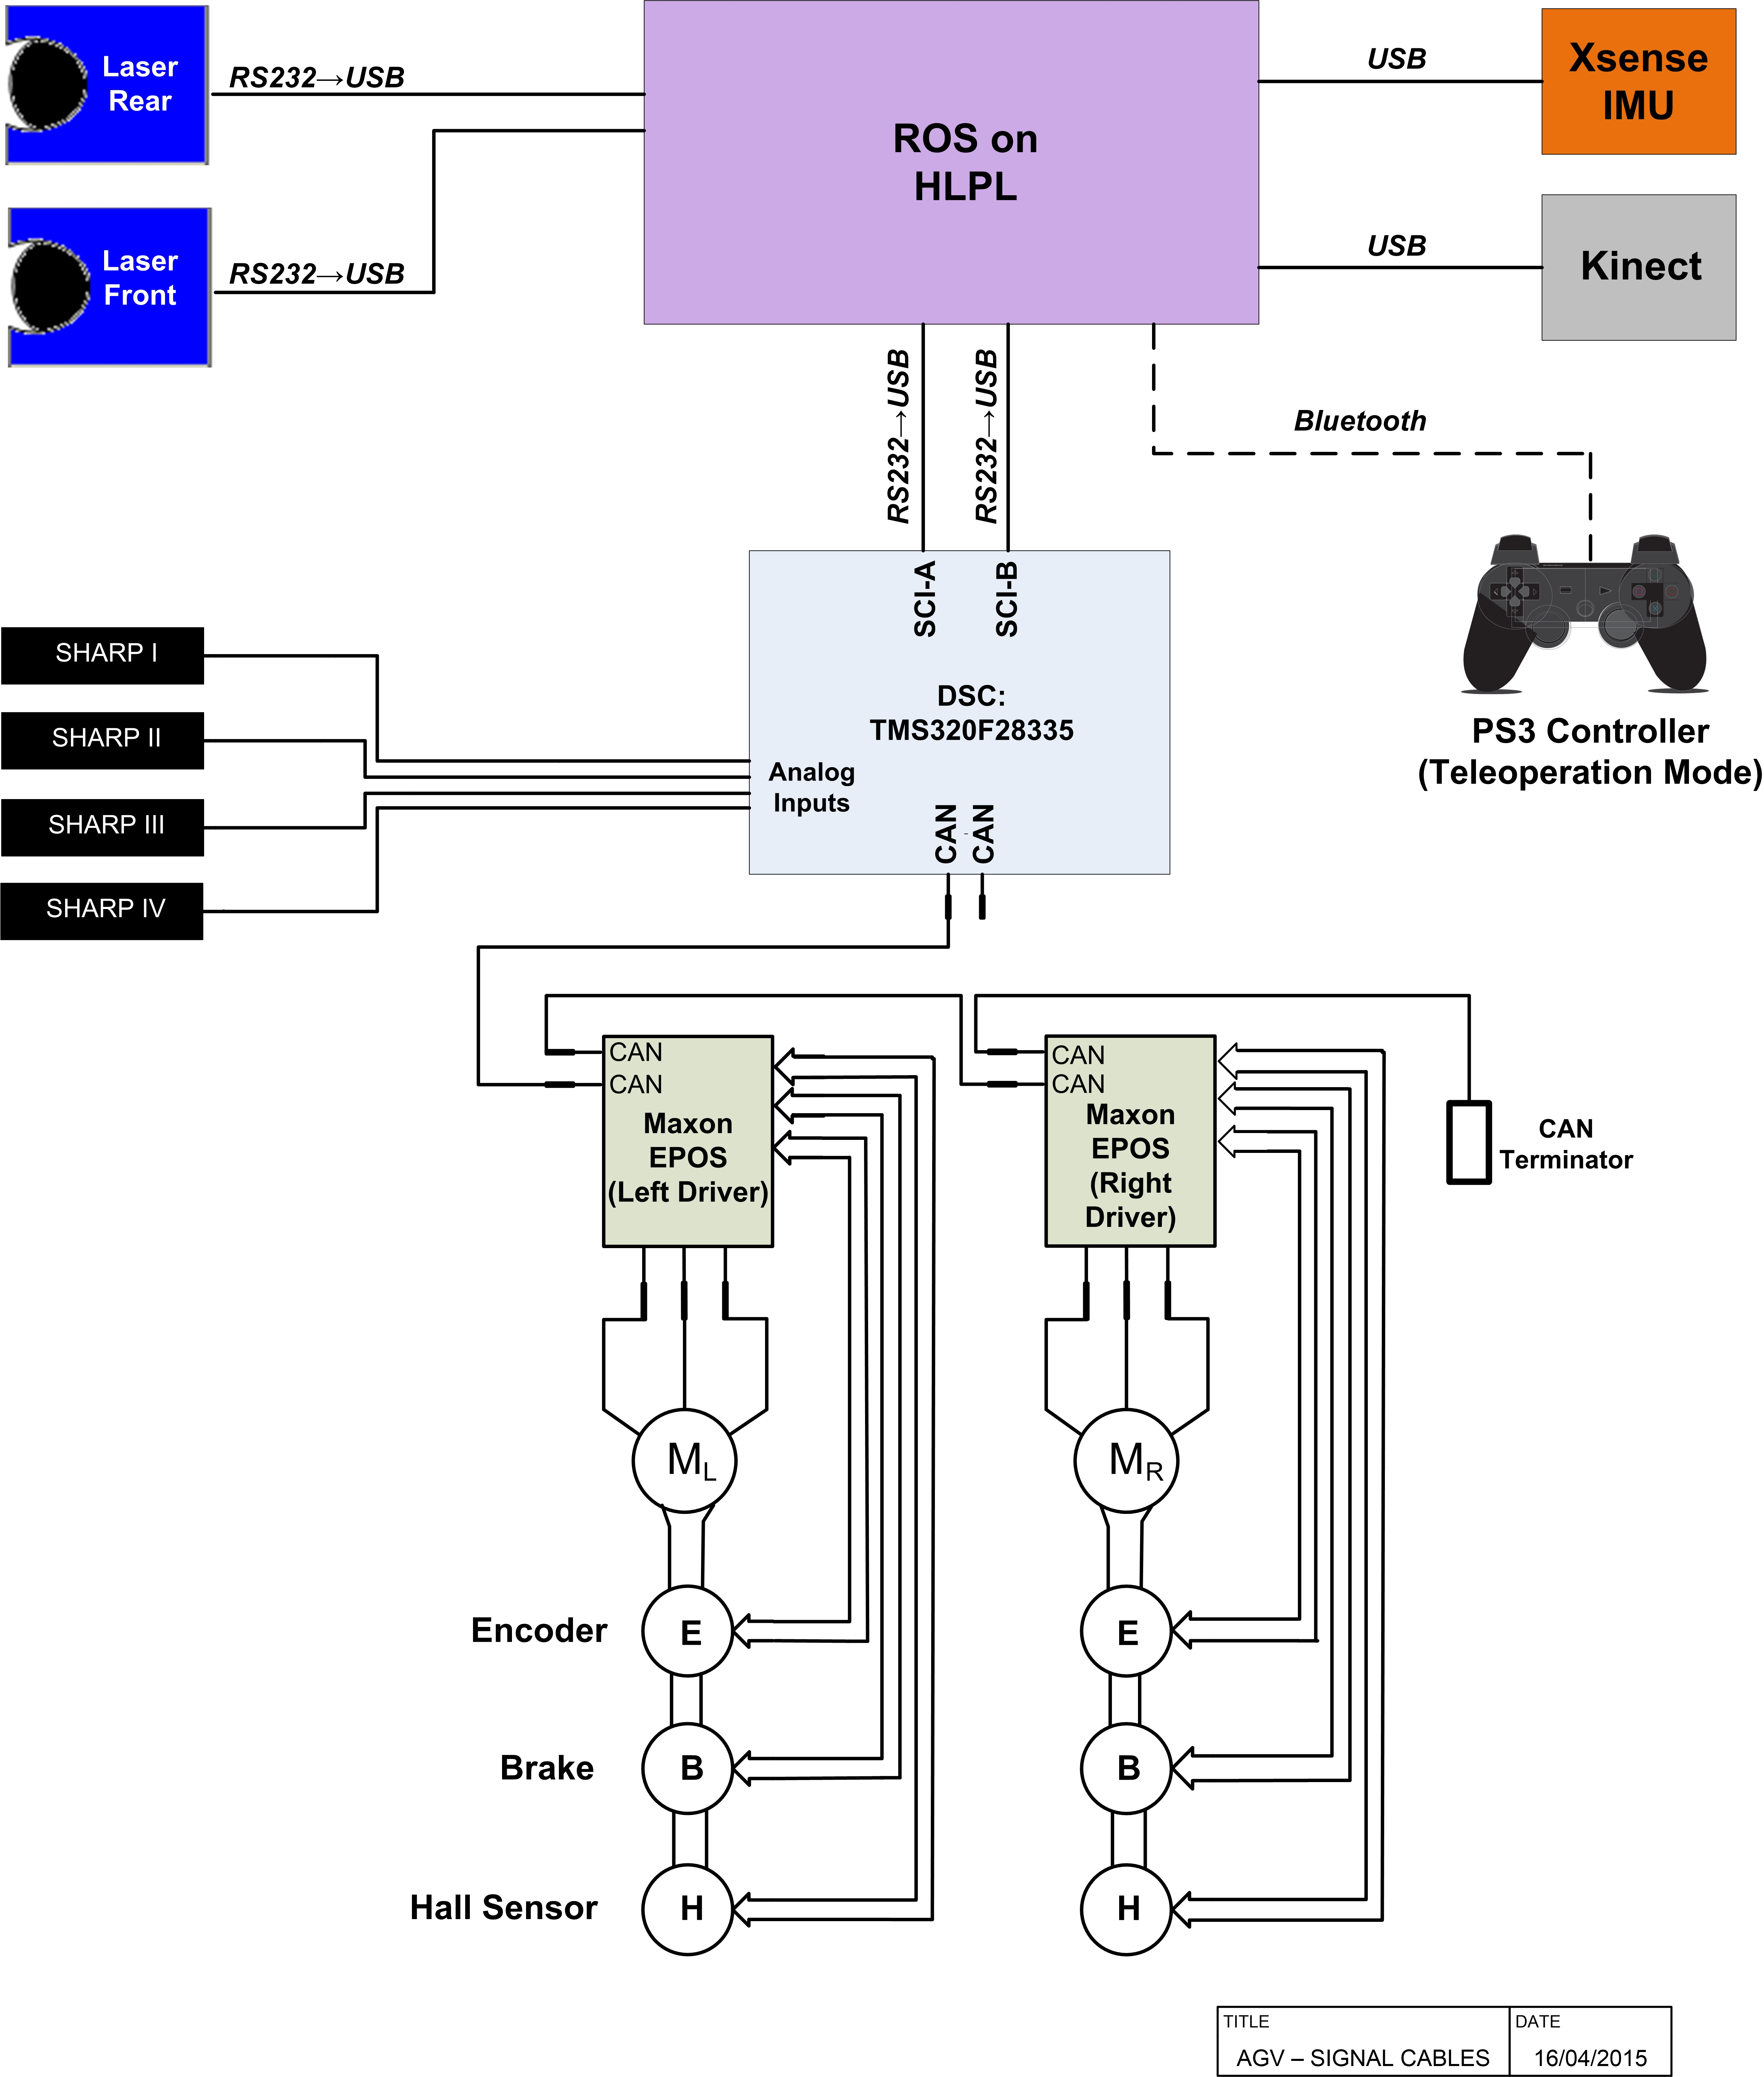
\includegraphics[scale=0.45]{images/agvSignal}
	\caption{Signal chart of ITU-AGVs}
	\label{fig:agvSignal}
\end{figure}

\section{Embedded Program Development for LLPL}
\label{sec:embedded dev}
The embedded software for TMS320F28335 microcontrollers at LLPL is developed using Simulink Embedded Target Coder in MATLAB r2012b and then the make files are uploaded to the microcontroller using TI Code Composer Studio v4. 
	\subsection{Communication with EPOS Drivers}
	\label{subsec:comm with epos}
	The Maxon EPOS 70/10 motor drivers are designed to be used with CANOpen protocol. In CAN communication several hardware are connected as slaves to a master using a CAN Bus. The communication and configuration occurs with using array of variables called objects. Object dictionary includes all object addresses with 16-bit index and 8-bit sub index. 
	\par
	EPOS drivers have their configurable controllers and there are several driving modes such as position mode, velocity mode, profile velocity mode and so on. It is desired to send velocity commands to the LLPL and to settle the motors on the desired velocity references. So the operation mode would be selected as the profile velocity mode. 
	\par
	According to the EPOS 70/10 Manual~\cite{eposManual}, the motors are controlled with given profile velocity and acceleration limits and selection of motion profile type. Motion profile type can be selected as linear or sinusoidal. It is desired to obtain a sinusoidal profile. In the manual, all configuration and communication object values and their places in the work flow are provided. 
	\par
	\begin{figure}[h]
		\centering
		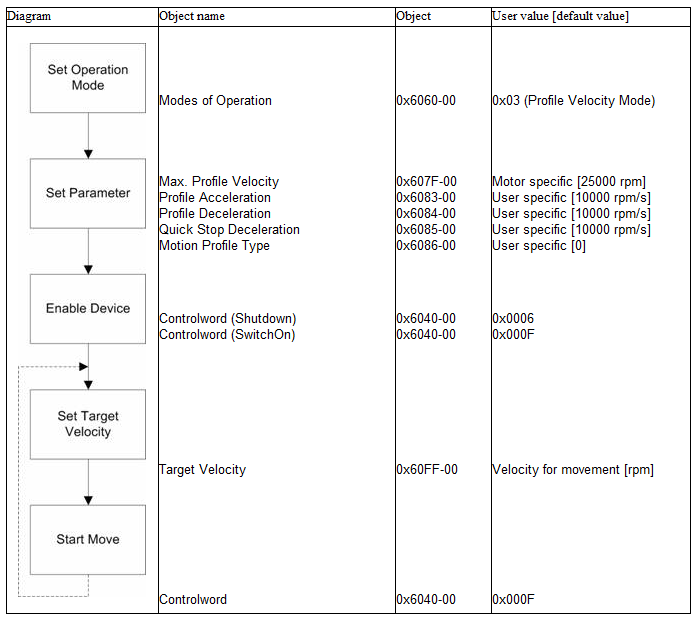
\includegraphics[scale=0.7]{images/eposProfileVelocity}
		\caption{Configuration flow chart for profile velocity mode ~\cite{eposManual}}
		\label{fig:eposProfileVelocity}
	\end{figure}
	In Simulink, a state chart diagram is created in order to make the program flow as a state machine. In the program, according to the EPOS 70/10 Manual the necessary configurations are being made. First, all CANOpen nodes are being reset and all slaves are being set as operational. Then according to the chart in Figure ~\ref{fig:eposProfileVelocity}, the operation mode is being selected as profile velocity mode, the values for maximum profile velocity, profile acceleration, profile deceleration, quick stop deceleration and motion profile type are being configured over their objects and a necessary reset is being done. After these configurations, the program enters a loop. In the loop, the commands are being taken from HLPL over SCI-A (Serial Communication Interface - A) serially. The commands are being parsed and left and right motor commands are separated and set as target velocity values. The control word is being sent and encoder values are being requested. After the encoder values are received, they are being sent to HLPL over SCI-B and the loop begins again. The flow of the state chart diagram in Simulink can be seen in Figure ~\ref{fig:simulinkStateFlow}.
	\begin{figure}
		\centering
		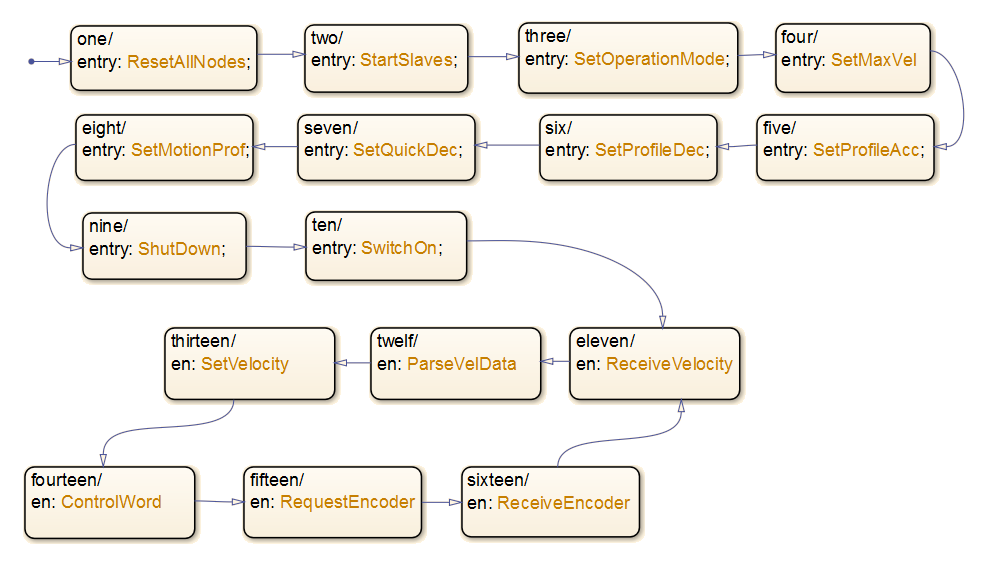
\includegraphics[scale=0.5]{images/simulinkStateFlow}
		\caption{State chart flow diagram of LLPL in Simulink}
		\label{fig:simulinkStateFlow}
	\end{figure}
	
	\subsection{Communication with HLPL}
	\label{subsec:comm with hlpl}
	The velocity commands are designed to be in one sixteenth of desired rpm values at the motor shaft before gear-box. LLPL takes commands in 16-bit integers. The command word will be sent starting with “\#” character and ending with “!” character. The first 16-bits after starting character will be the left motor command and the second 16-bits until the end character will be the right motor command. Commands are 16-bits and the first byte of each command is for direction and the second byte is for one sixteenth of the rpm value desired at the motor shaft before the gear-box. Before sending the values to the drivers, this value is multiplied by. It is important to remind the gear-box on the motor since it reduces the rpm with a ratio of 1:100. 
	\par
	For example, if it is wanted to drive the wheels at 40 rpm, a basic calculation can be made. The rpm value at the shaft of the motor before the gear-box would be $40\times100=4000$. This is the target rpm value, so the second byte of the command must have the value of $4000\div16=250$. 
	\par
	The direction is set such that, if the value of the direction byte is less than or equal to 127 it is counted as positive direction and the otherwise is negative direction. So the necessary word needed to be send to LLPL in order to drive wheels at 40 rpm in the positive direction should be 
	$[\#\text{0 250 0 250}!]$. The parsing is made in then made in LLPL. 
	\par
	EPOS 70/10 can provide various calculations with encoder values and it can give position and velocity. The encoder values are being sent in 16-bits to HLPL. Both SCI-A and SCI-B serial communications are set at 115200 baud.
		
	\subsection{Testing the LLPL}
	\label{subsec:testing llpl}
	In order to test the embedded software and the serial communication a simple test script is written with Python. In the script the direction and desired wheel rpm values are requested from the user for left and right wheels and the command word is calculated and sent over serial port to the ITU-AGVs (Figure ~\ref{fig:testScript}). After using this test script, it is concluded that the LLPL is functionally working and the project can be moved on to HLPL.
	
	\begin{figure}[h]
		\centering
		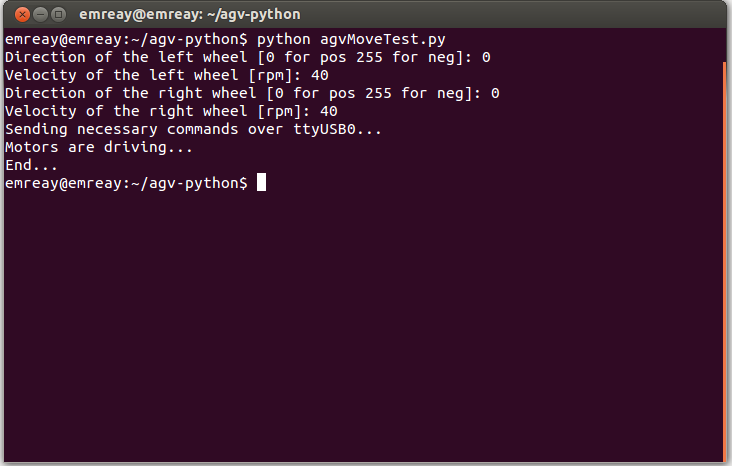
\includegraphics[scale=0.65]{images/testScript}
		\caption{Testing LLPL with a written Python script}
		\label{fig:testScript}
	\end{figure}
	
\section{ROS Programming for HLPL}
\label{sec:programming for hlpl}

	\subsection{ROS Installation \& System Initialize}
	\label{subsec:ros install and init}
	Pre-compiled repositories for ROS distributions are officially supported and supplied for Ubuntu. The HLPL would be ROS running on Ubuntu 12.04 LTS on a notebook computer. ROS Groovy distribution is supported on Ubuntu 12.04 LTS so its complete packages are installed according to the directives at ROS Wiki Website. 
	\par
	After installation a workspace is needed to be created. Workspace is the container folder where all the packages and their relative files are stored. Catkin build system has a command to easily create a workspace for ROS. 
	\par
	There are several packages needed to be installed that are not included in the ROS core packages. These are usually specific work or hardware packages. Since the sensors to be installed are decided, their relative software driver packages for ROS are installed including ps3joy for Play Station 3 joystick, sicktoolbox wrapper for laser sensors and xsens driver for IMU. 
	\par
	To contain the applications that are going to be written, a ros package is needed to be created. Catkin also provides an easy package creation with a command and its several arguments. Packages usually depend on other packages in order to use their functionalities. So a package named \textit{agv} is created with dependencies to \textit{roscpp} and \textit{rospy} packages. This package together with all the written ROS codes in this project is available at the link given in Appendix ~\ref{appendix}.
	\subsection{Teleoperation Application}
	\label{subsec:teleop app}
	Teleoperation is a vital functionality for manual data collection or to move the robot to the application areas. It is needed to be able to move ITU-AGVs manually as desired in order to collect laser data or images for use in algorithm development on Simultaneous Localization and Mapping (SLAM), loop closure or similar applications. 
		\subsubsection{Simulation}
		\label{subsec:simulation}
		Before directly passing to work on ITU-AGVs, the teleoperation is desired to be applied on a simulation environment of ROS. To achieve this, a visual model has to be created. Rviz visualization environment supports an xml based format for basic 3D robot representation called Unified Robot Description Format (*.urdf). It is a simple parser with a simple syntax. So basically, a box with to wheels in the dimensions and placement of the ITU-AGVs can be created by a urdf file as follows;
		\lstinputlisting[title={Urdf code for ITU-AGVs}]{codes/agv_.urdf}
		So basically the links and joints are geometrically defined with their positions, dimensions together with their relationship with each other. So their hierarchy tree can be understood by the system and it is possible to visually see the tree as in Figure ~\ref{fig:urdfTree}. When the created urdf file is opened in Rviz, a simple box and two wheels with the given parameters can be seen as in Figure ~\ref{fig:agv-urdf}. This visualization is a simple and quick solution. But it is possible to integrate more realistic 3D models. Rviz supports Collada file format (*.dae) which is an open xml schema, so the 3D models created in various CAD software such as Google SketchUp can be converted to Collada file and implemented to Rviz~\cite{Martinez-Ros}. So a 3D model of ITU-AGVs are created using Google SketchUp and it is converted to the Collada file (Figure ~\ref{fig:agv-dae}).
		\begin{figure}[h]
			\centering
			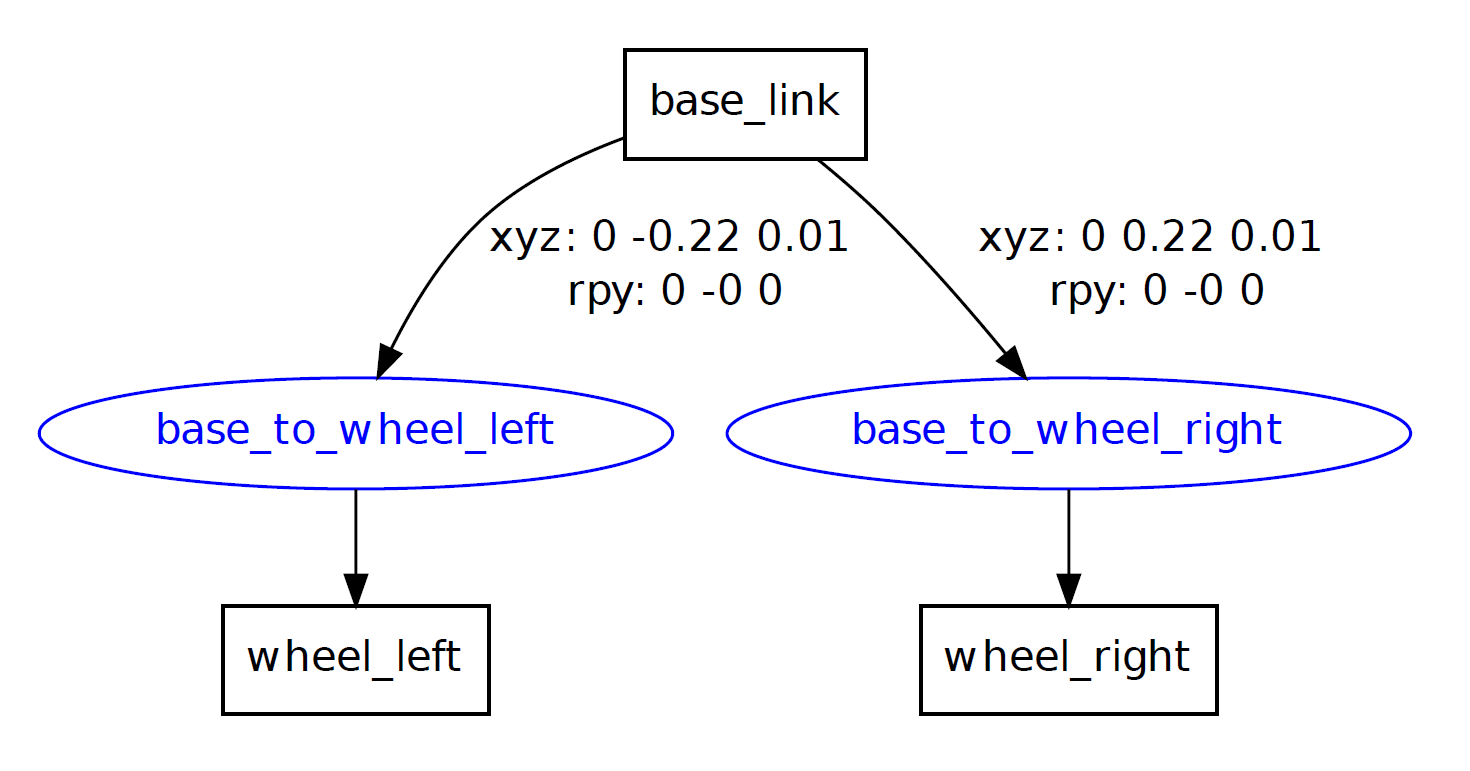
\includegraphics[scale=0.3]{images/urdfTree}
			\caption{Urdf tree}
			\label{fig:urdfTree}
		\end{figure}
		
		\begin{figure}[h]
			\centering
			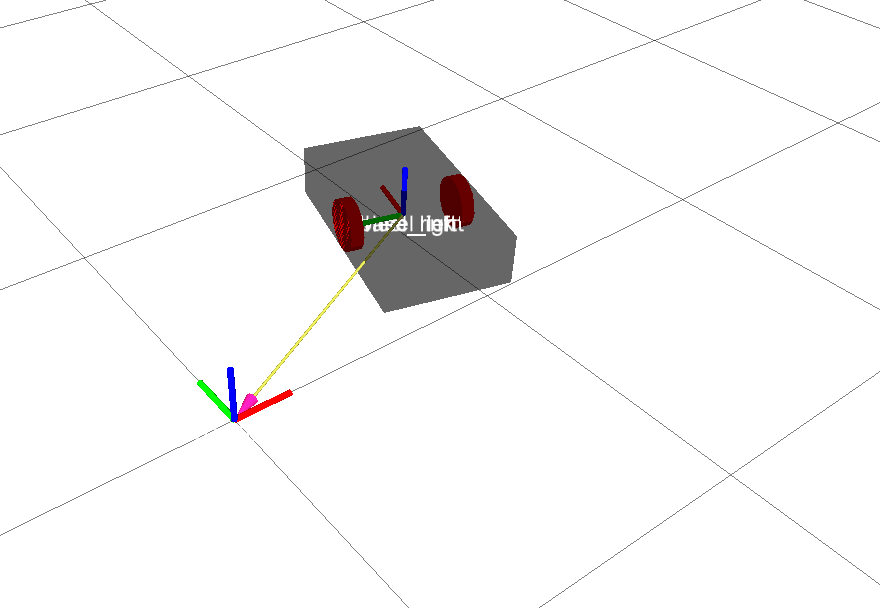
\includegraphics[scale=0.55]{images/agv-urdf}
			\caption{Urdf model of ITU-AGVs}
			\label{fig:agv-urdf}
		\end{figure}
		\par
		It is wanted to realize the tele-operation using the Play Station 3 joystick. It is desired to control with both analog buttons and digital buttons. In the analog mode, the vertical values of left and right analog buttons will be the angular velocity references (in rpm) of left and right wheels. In digital mode, cross buttons will drive the motors on constant angular velocities. The up and down direction buttons will move the robot forwards and backwards, left and right buttons will drive the motors in the opposite directions resulting in a clockwise and a counter clockwise rotation around the central point. Lastly it is desired to only one mode at a time, hence while R2 button on the joystick is pushed digital mode would be active and otherwise analog mode would be active. 
		\par
		\begin{figure}[h]
			\centering
			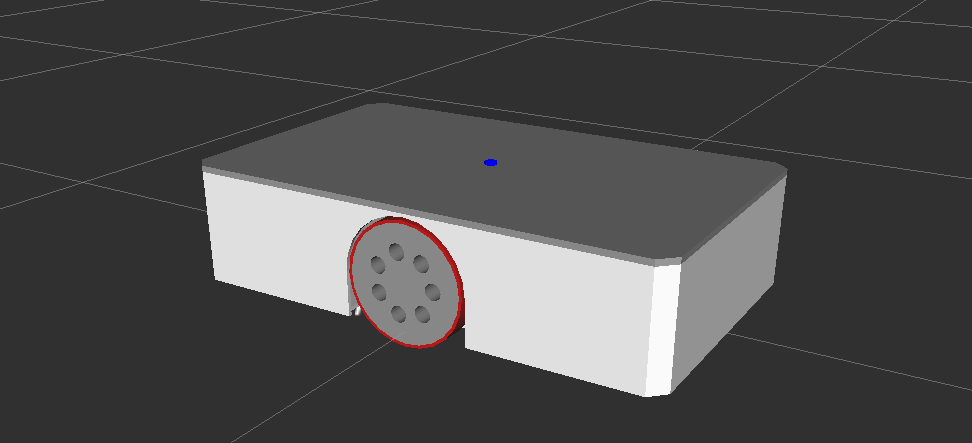
\includegraphics[scale=0.5]{images/agv-dae}
			\caption{3D model ITU-AGVs opened in Rviz}
			\label{fig:agv-dae}
		\end{figure}		
		Using the installed ps3joy package, communication with PS3 joystick over Bluetooth is handled and the button values are published to ROS environment. A node that subscribed to the joystick topic is created. This node gets the joystick button values, and passes the values of the necessary buttons as the relevant joint’s velocity with multiplying it with a scalar, then publishes all the joint states. Another node is written so that it is subscribed to the topic that joint states are published. When the joint states data is received this node passes the velocity data to the parameter server in the callback function. Then in the main loop, it calculates the odometry of the robot and publishes the odometry information. 
		\par
		After building the nodes and launching them the 3D model of ITU-AGVs have successfully moved with using the PS3 joystick (Figure ~\ref{fig:agv-teleop-sim})	
		\begin{figure}[h]
			\centering
			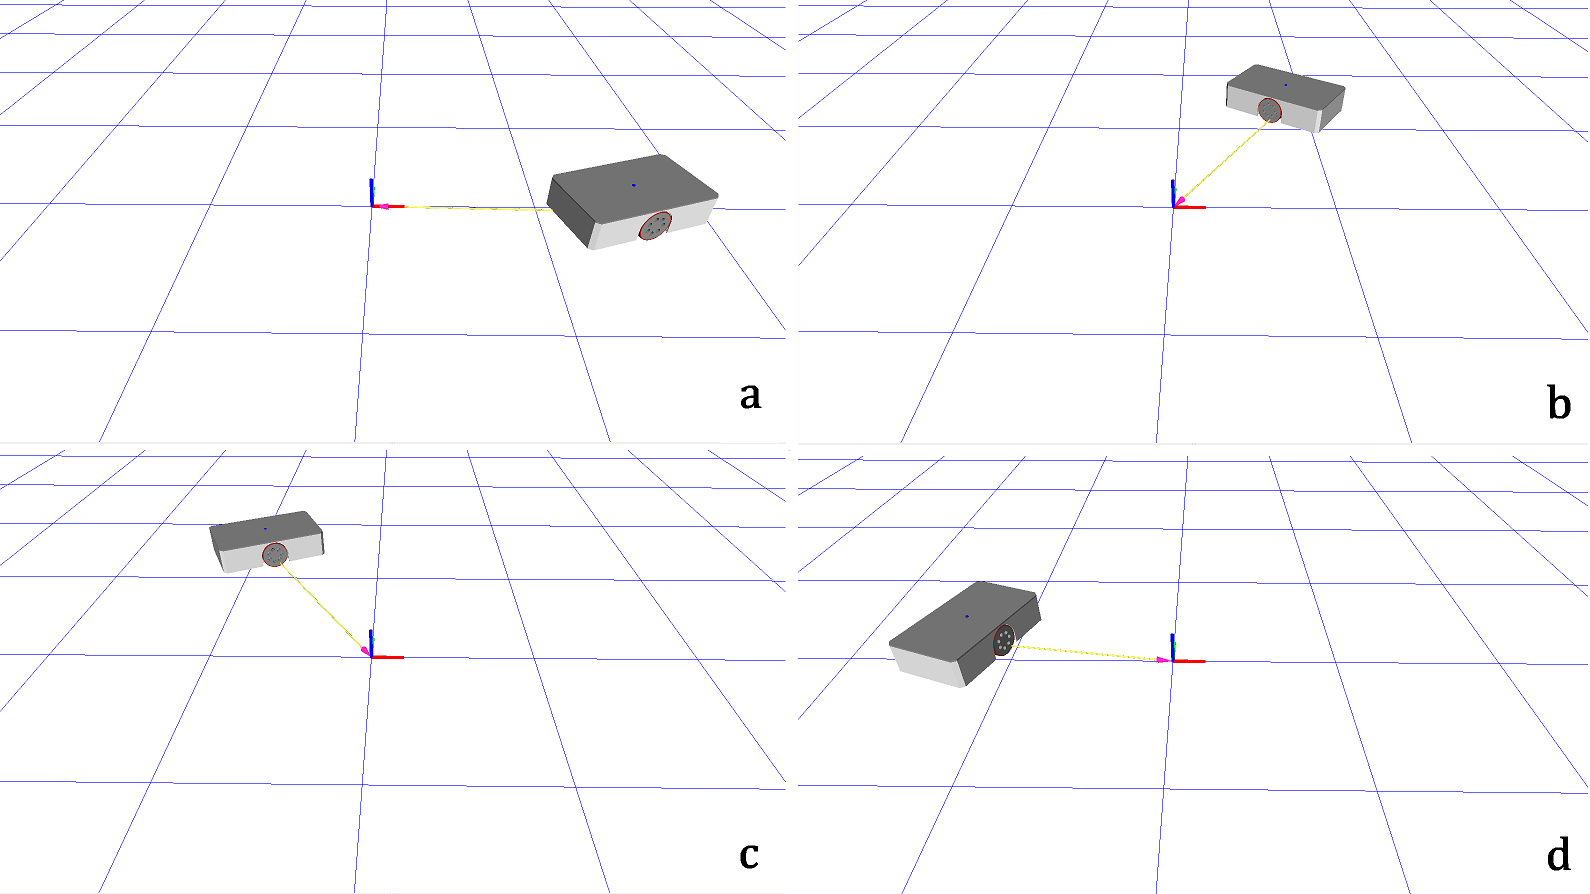
\includegraphics[scale=0.3]{images/agv-teleop-sim}
			\caption{Teleoperation of ITU-AGV model in Rviz}
			\label{fig:agv-teleop-sim}
		\end{figure}		
		\subsubsection{Teleoperation of ITU-AGVs}
		\label{subsec:teleop pkg}
		Since the teleoperation is successfully made on the simulation, it is convenient to realize the teleoperation of ITU-AGVs. A similar but modified approach is made. A node is created so that it would subscribe to the joystick topic and every time the joystick data is received it takes the needed button values. If the R2 button is pressed, it configures several variables depending on the values of digital cross buttons. If R2 button is not pressed, it configures the same variables depending on the analog button values. In the main loop, the node publishes an array of the variables which are configured in the callback function. This array is in the form that has been specified in Section ~\ref{subsec:comm with hlpl}. In order to send the commands to ITU-AGVs, another node is subscribed to the topic in which the array is published and it sends the array to LLPL of ITU-AGVs over a serial COM port. After the nodes are built, teleoperation of ITU-AGVs is successfully achieved. Node graph is shown for the teleoperation in Figure ~\ref{fig:teleop-graph}. It is possible to see the node graph in ROS in order to examine the relationships of nodes over topics and to see which nodes and topics are active. This is a powerful feature for diagnostics. 
		\begin{figure}[h]
			\centering
			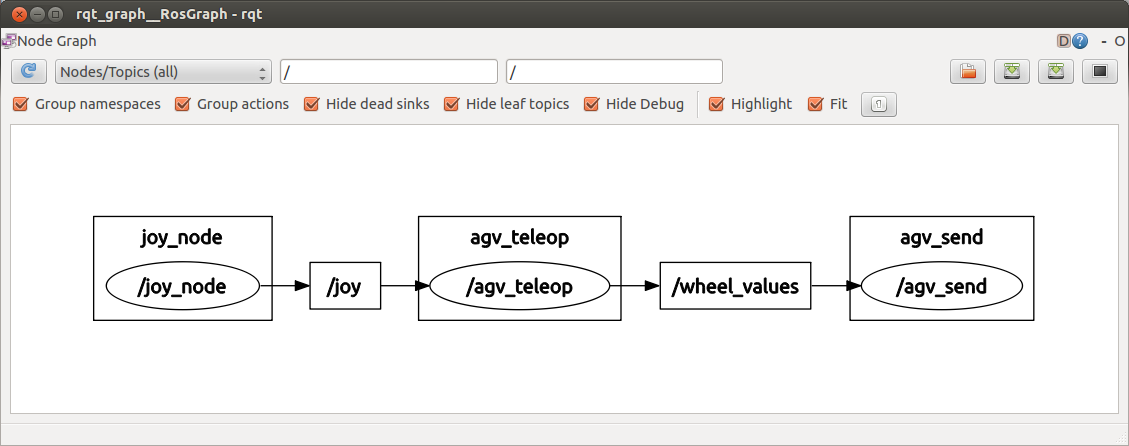
\includegraphics[scale=0.43]{images/teleop-graph}
			\caption{Node graph (rqt-graph) of teleoperation}
			\label{fig:teleop-graph}
		\end{figure}
	\subsection{Sensor Integration}
	\label{subsec:sensor integration}
	Software packages of various sensors were installed during the system initialize. Since the teleoperation is applicable, reading stable data from the sensors on ROS is the next goal. 
		\begin{figure}[h]
			\centering
			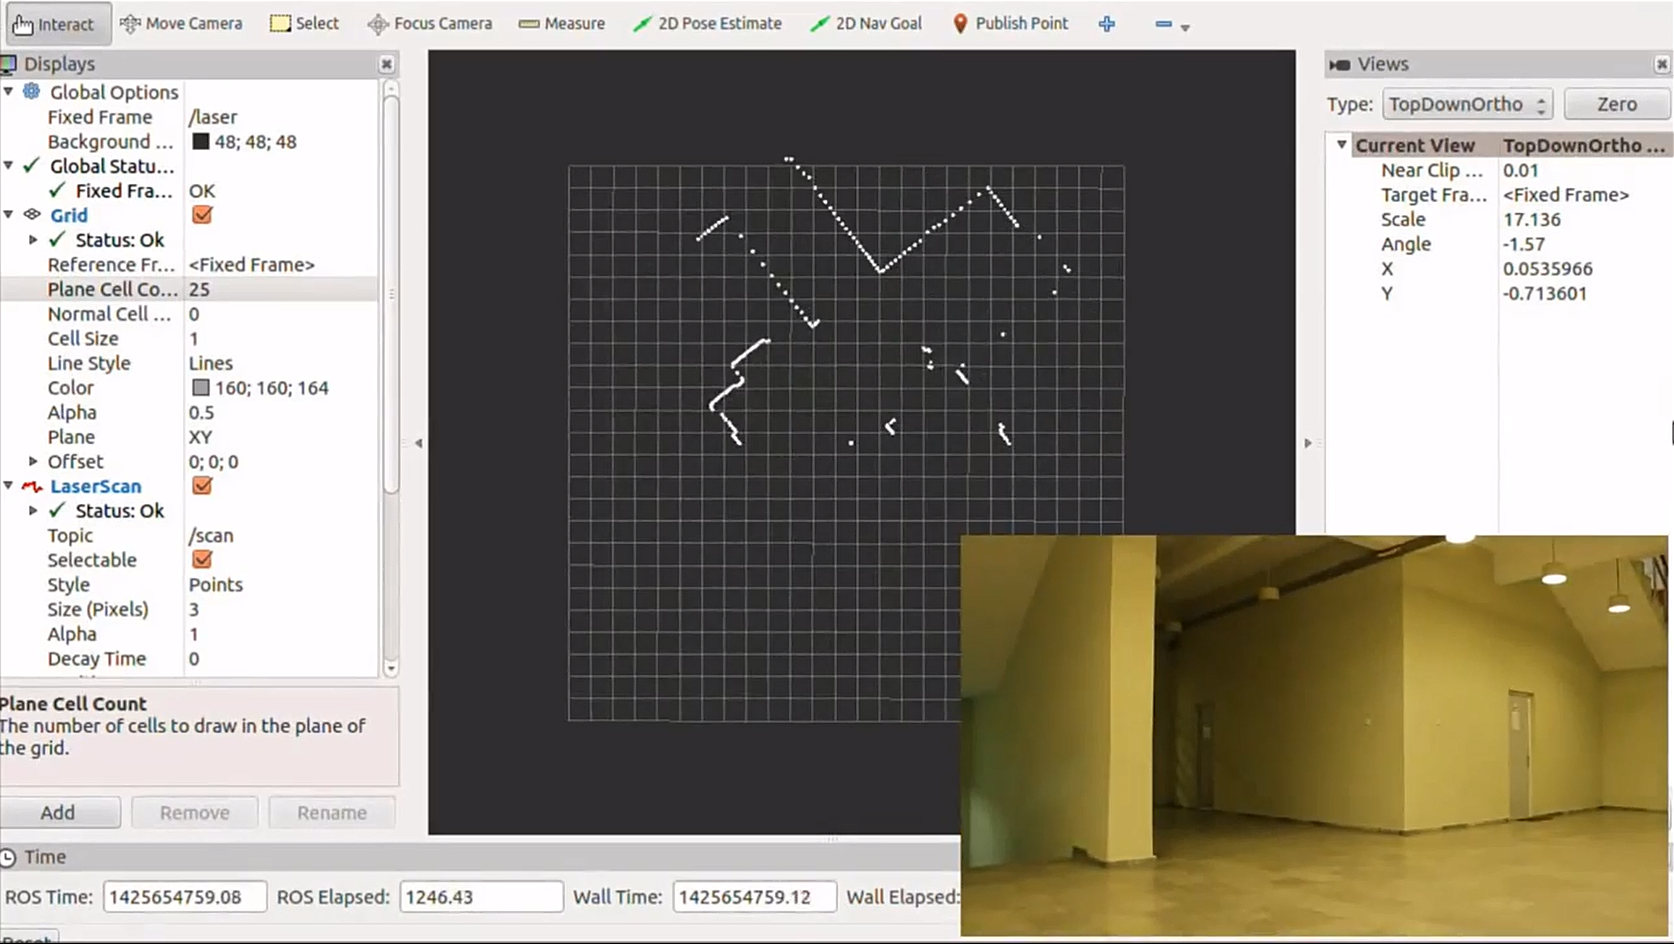
\includegraphics[scale=0.3]{images/lidar-sim}
			\caption{Simultanoues stream of LIDAR data on Rviz and the image of real environment}
			\label{fig:lidar-sim}
		\end{figure} 
		\subsubsection{Encoder Reading}
		\label{subsec:encoder reading}
		The encoder values are sending over SCI-B as they have configured to do in Section ~\ref{subsec:comm with hlpl}. In the HLPL, they have to be read. To read the encoder values, a Python node is written. In this node, the COM port assigned to SCI-B (ttyUSB1) is continuously listened. Since the sending format is the same (start character as “\#”, end character “!”), the node converts the unsigned 16-bit integer values to signed 16-bit values and publishes the converted values on a topic. 
		\subsubsection{IMU Reading}
		\label{subsec:imu reading}		
		The related ROS package for Xsens MTi IMU was installed before. Using this package a launch file is created and the node that publishes IMU data is successfully initialized. In order to calibrate the data and make certain settings the software provided by Xsens is used. As shown in Figure ~\ref{fig:xsens-test}, the robot is rotated around its center for approximately 90 $^{\circ}$ clockwise and counter clockwise and the yaw angle is plotted from the IMU data. It can be also seen that the robot settles smoothly in sinusoidal profile as the motor drivers are configured to do in Section ~\ref{subsec:comm with epos}.
		\begin{figure}[h]
			\centering
			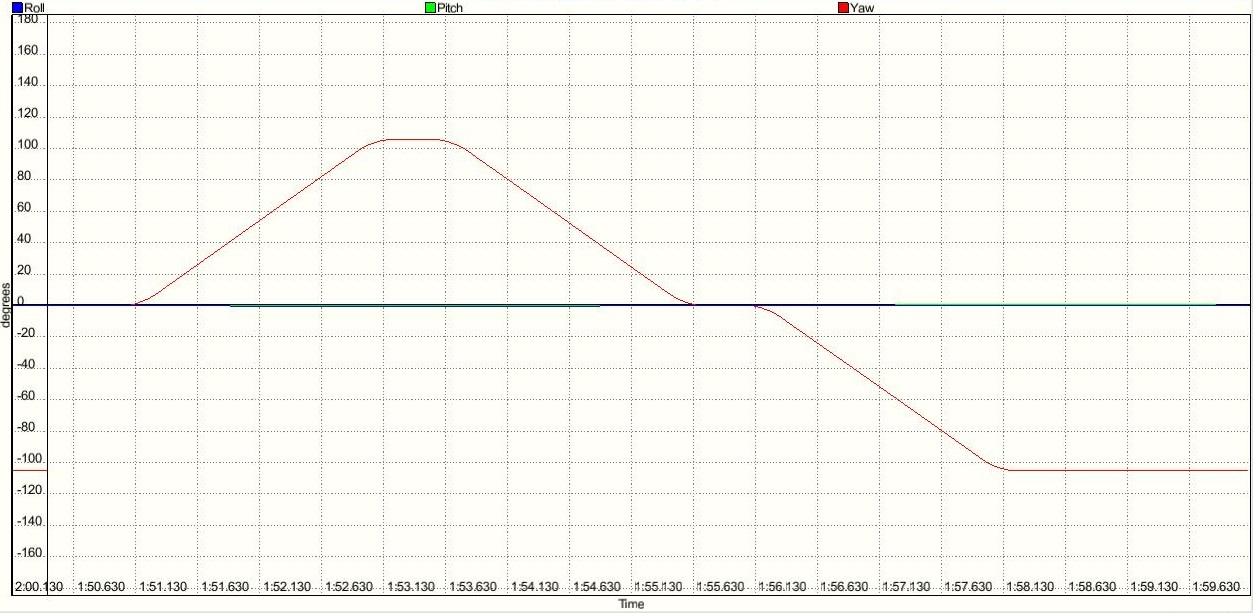
\includegraphics[scale=0.4]{images/xsens-test}
			\caption{Yaw angle values is retrieved from IMU while the robot is rotating}
			\label{fig:xsens-test}
		\end{figure} 	
		\subsubsection{LIDAR Reading}
		\label{subsec:lidar reading}	
		The related package publishes laser scan data on ROS environment. A launch file is created and the data scanned by the LIDAR is simultaneously published on Rviz as in the Figure ~\ref{fig:lidar-sim}.	
		\subsubsection{Kinect Reading}
		\label{subsec:kinect reading}		
		OpenNI driver packages for Kinect are installed. After a launch file is created, both RGB and point cloud data are streamed to Rviz (Figure ~\ref{fig:kinect-pcl}).
		
	\subsection{Odometry Estimation}
	\label{subsec:odom estimation}
	Odometry estimation is a vital step since it is not possible to robot to autonomously move, navigate and plan without the information of its position and orientation with respect to the environment. The basic odometry calculation is made using the left and right wheel velocities obtained from the motor encoders. However, this calculation alone might give inexact or wrong odometry information due to errors in the calculation of velocity or slippage of the robot wheels.
		\begin{figure}[h]
			\centering
			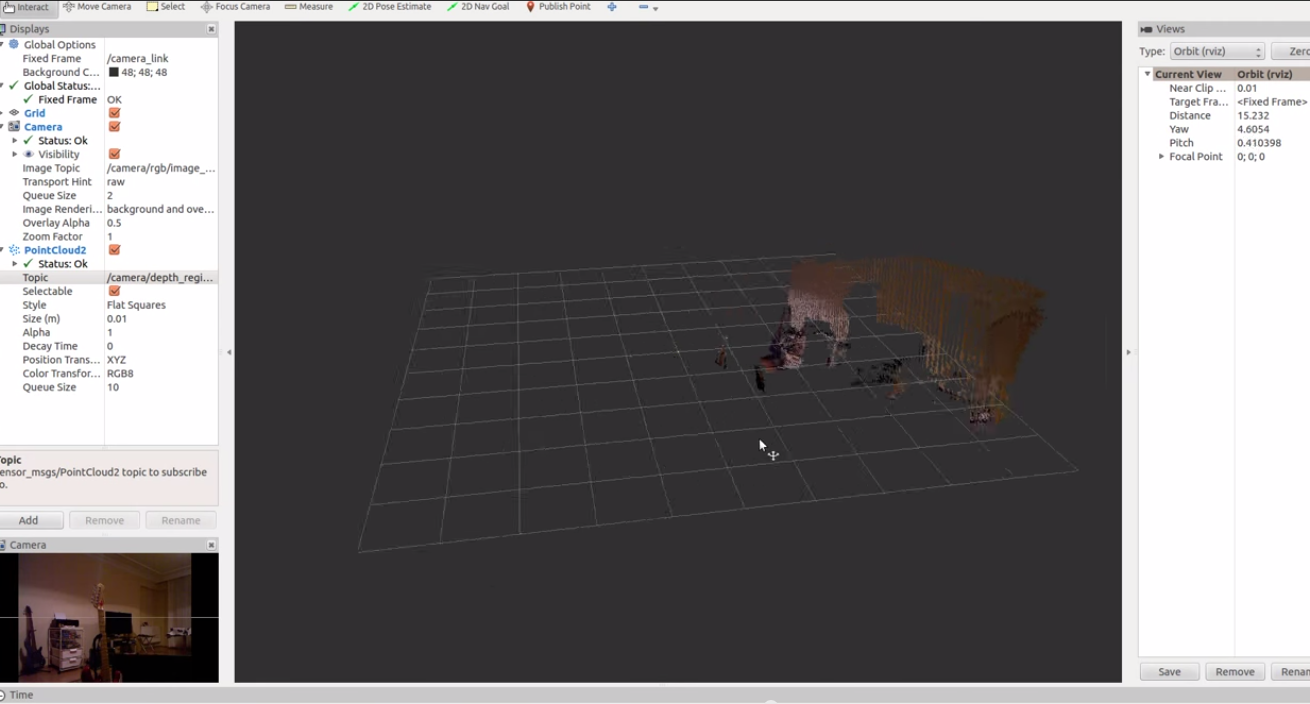
\includegraphics[scale=0.38]{images/kinect-pcl}
			\caption{RGB and point cloud data stream from Kinect on Rviz}
			\label{fig:kinect-pcl}
		\end{figure}	
	\par
	To get better and more reliable odometry information, the present-day robotics systems use IMU data or vision along with the encoders. The process called data fusion is applied in these cases to integrate various data. There are various advanced methods for multi-sensor data fusion which are beyond the scope of this project. However, there is a ROS package that provides data fusion for IMU and encoder data to estimate the pose of a robot using Extended Kalman Filter (EKF) named robot pose ekf  ~\cite{robotPoseEkf}. 
	\par
	Extended Kalman Filter in this case estimates an optimal value for odometry from the data of IMU and encoder and with a covariance matrix that tells how much accurate the data are. Using robot pose ekf package, the fused odometry information can be obtained. The necessary launch file is created so the nodes that publish IMU data and encoder values are started and the fused odometry information is published on a topic. The node graph can be seen in Figure ~\ref{fig:ekf-graph}.

	\begin{figure}
		\centering
		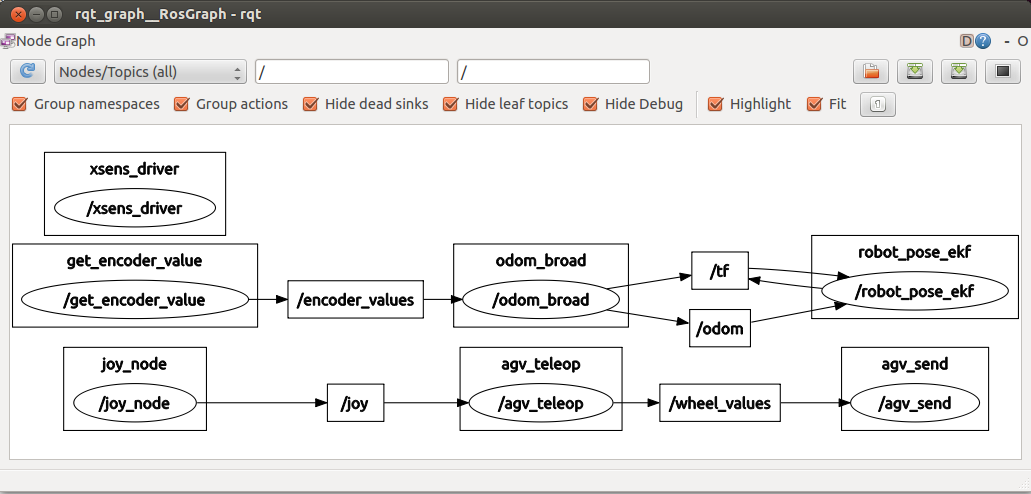
\includegraphics[scale=0.42]{images/ekf-graph}
		\caption{Node graph (rqt graph) while the robot pose ekf is publishing fused odometry data}
		\label{fig:ekf-graph}
	\end{figure}
				 
	\subsection{Offline Map Building}
	\label{subsec:offline mapping}					
	It is desired to build maps using collected data from the indoor environment. ROS can record and replay messages with makes it suitable for data collection. Since the odometry of ITU-AGVs can be estimated, sensors are installed, working and ready to publish data on ROS environment it is now possible to collect the necessary data while moving the ITU-AGVs to the desired areas. 
	\par
	A launch file for activating the nodes for IMU and encoder reading, odometry calculations and laser reading is created. 
	ROS records data to bag files and it is very simple to record desired or all topics that are active at the time of record. In this case the laser data and fused odometry information is needed to build a map. One of the ITU-AGVs is moved using Play Station 3 joystick while the selected topics are recorded inside ITU Electric and Electronics Faculty. After the data collection is done, the recorded data is replayed and using another package called gmapping an offline map of Control and Automation Department corridor is built as shown in Figure ~\ref{fig:map}.
	\begin{figure}
		\centering
		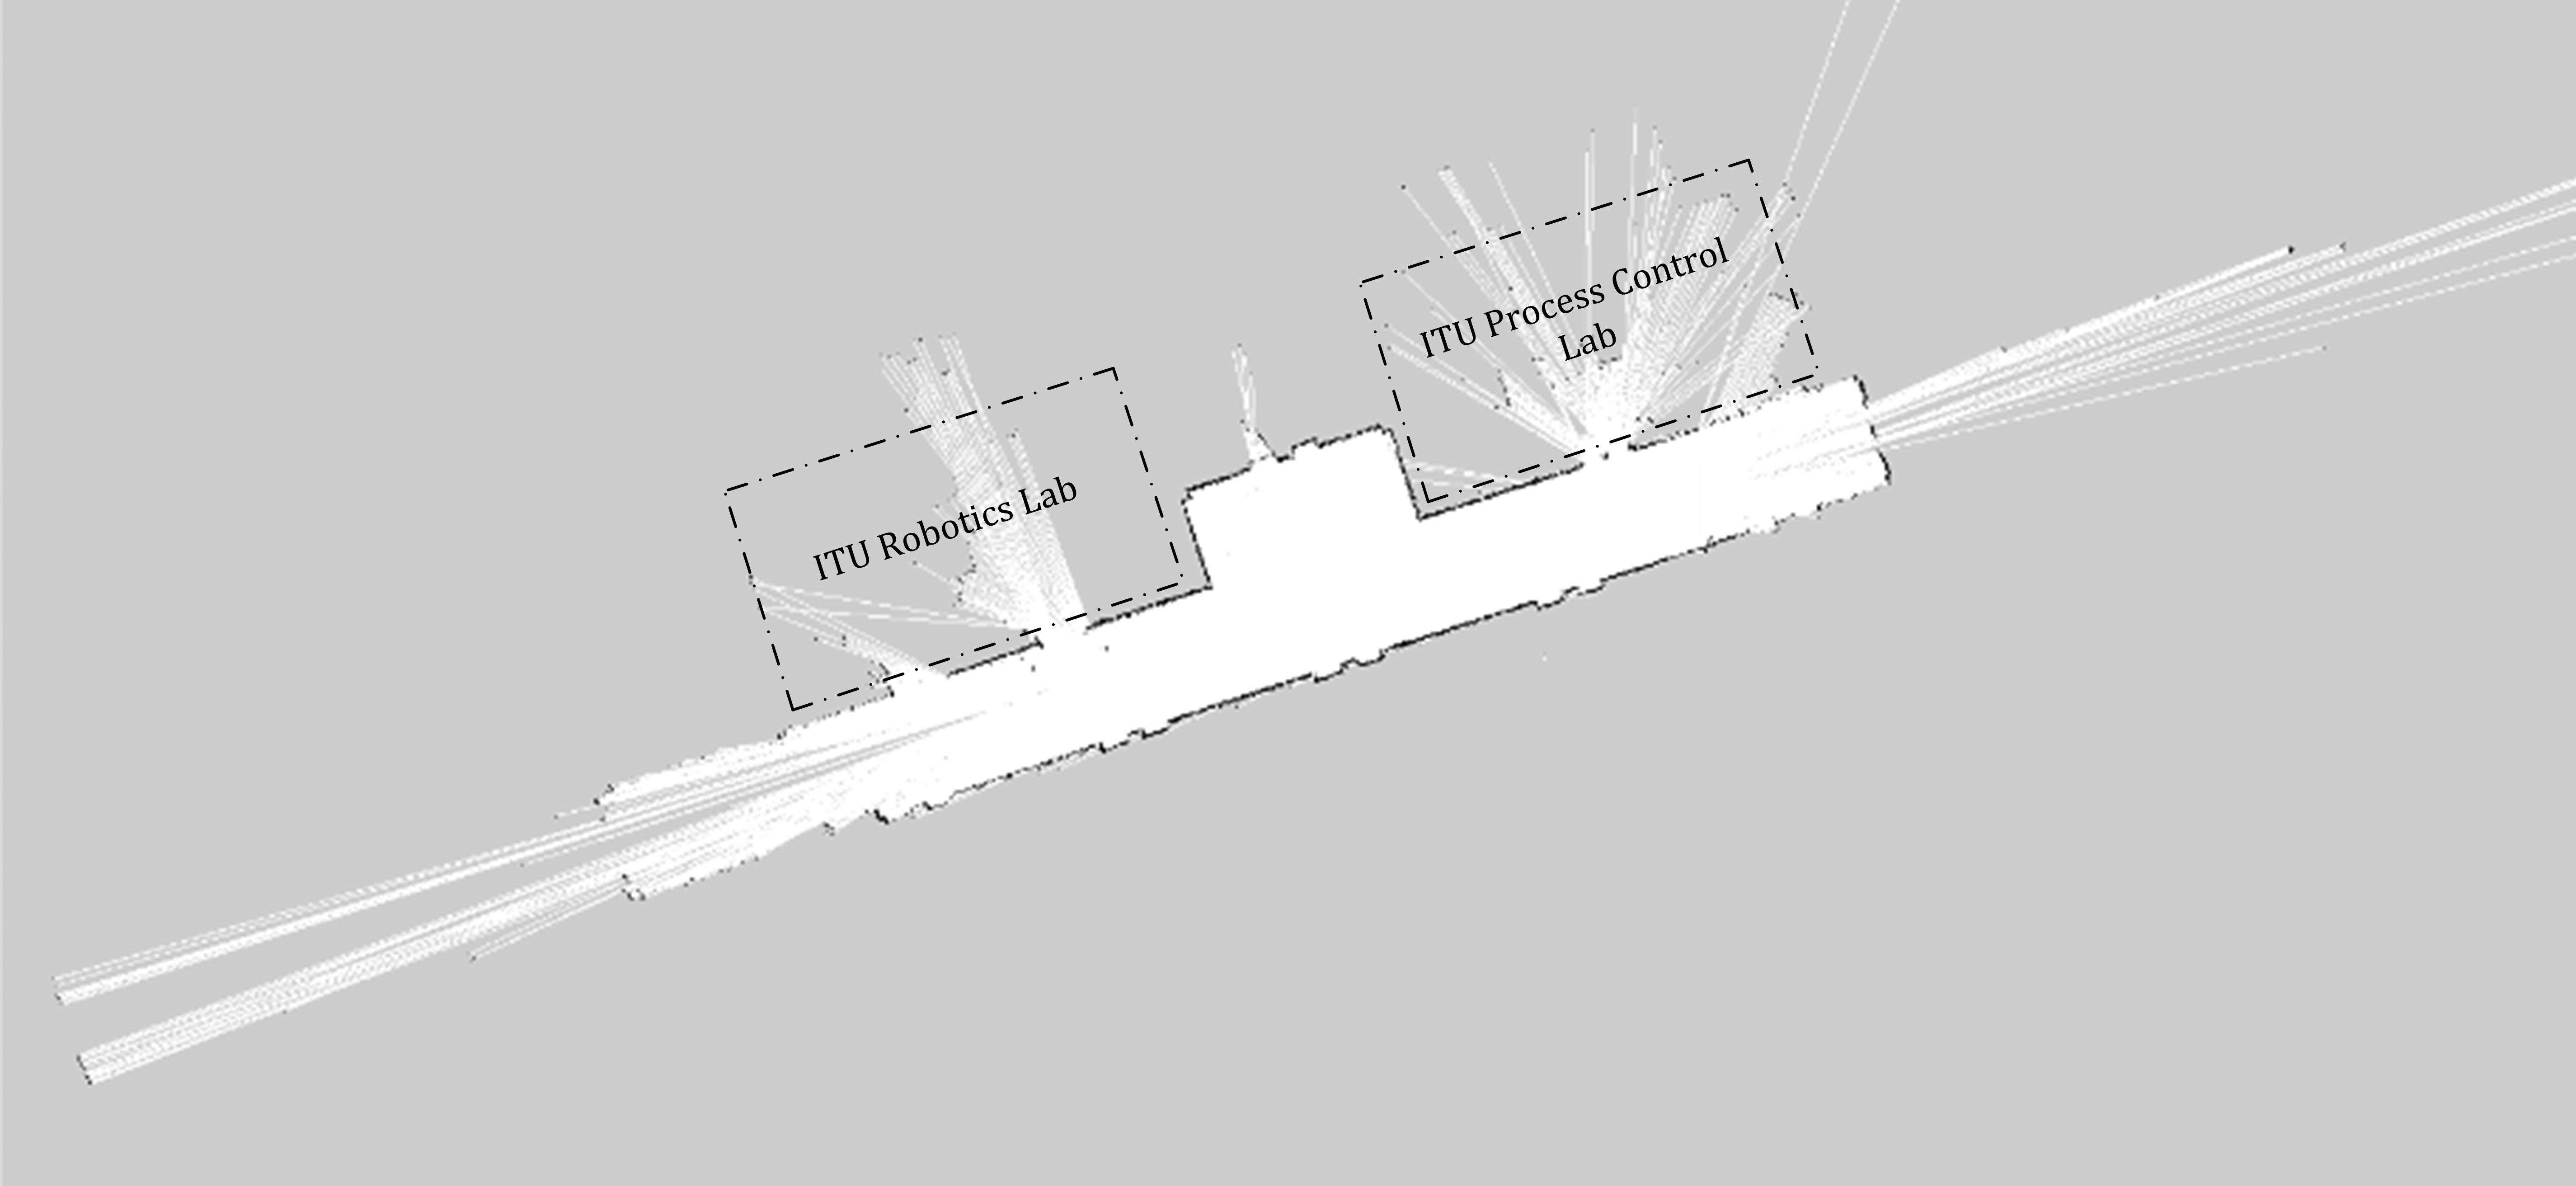
\includegraphics[scale=0.53]{images/map}
		\caption{An offline map of ITU Control and Automation Eng. Department corridor is built with the collected data}
		\label{fig:map}
	\end{figure}				
% Some commands used in this file
%\newcommand{\package}{\emph}

\chapter{Conclusion \& Future Work}
\label{chap:conclusion}
During the project, the necessary maintenance is made for ITU-AGVs, new embedded software is developed and it is designed to be ready for communication with ROS. A ROS package is created for ITU-AGVs which contain all the source codes, scripts, launch files, urdf files and custom messages. A 3D model is built for use in visual simulations and representation, the created model is implemented in ROS environment. It is possible in the future to use this model for simulation of navigation, SLAM, multi-robot system and various trials that would be subject of other theses, works or learning projects at ITU Robotics Laboratory. 
\par
ITU-AGVs are equipped with numerous sensors, and all the sensors are ready to be used, their sensor packages are installed and tested, launch files for different sensor combinations are created. 
\par
Teleoperation application is developed and tested. ITU-AGVs can simply be moved using a joystick. This would help to transport the robots to the desired application areas as well as data collecting. Thesis students who only focuses on certain data processing on a moving robot, i.e. RGBD or laser data, does not need to deal with the background process. They can directly do the teleoperation. 
\par
The vital step of acquiring odometry information is done. This information is directly provided for future studies that strictly depend on it. 
Lastly an offline map is built by recording selected data and combining them. This is the first part into mapping and it should be continued to autonomously online mapping. 
\par
The necessary basis is formed as desired with both embedded and computer software. This solved the problem of ITU-AGVs for being out-of-date and made a contribution to ITU Robotics Laboratory. 
\par
Based upon this work, many improvements can be initiated in the future. The created ROS package is a prototype since the process of learning proceeded in parallel with the project. The package can be separated into specific packages, and a metapackage for them can be created. The codes can be review in order to use in newer distributions of ROS. 
	\begin{figure}
		\centering
		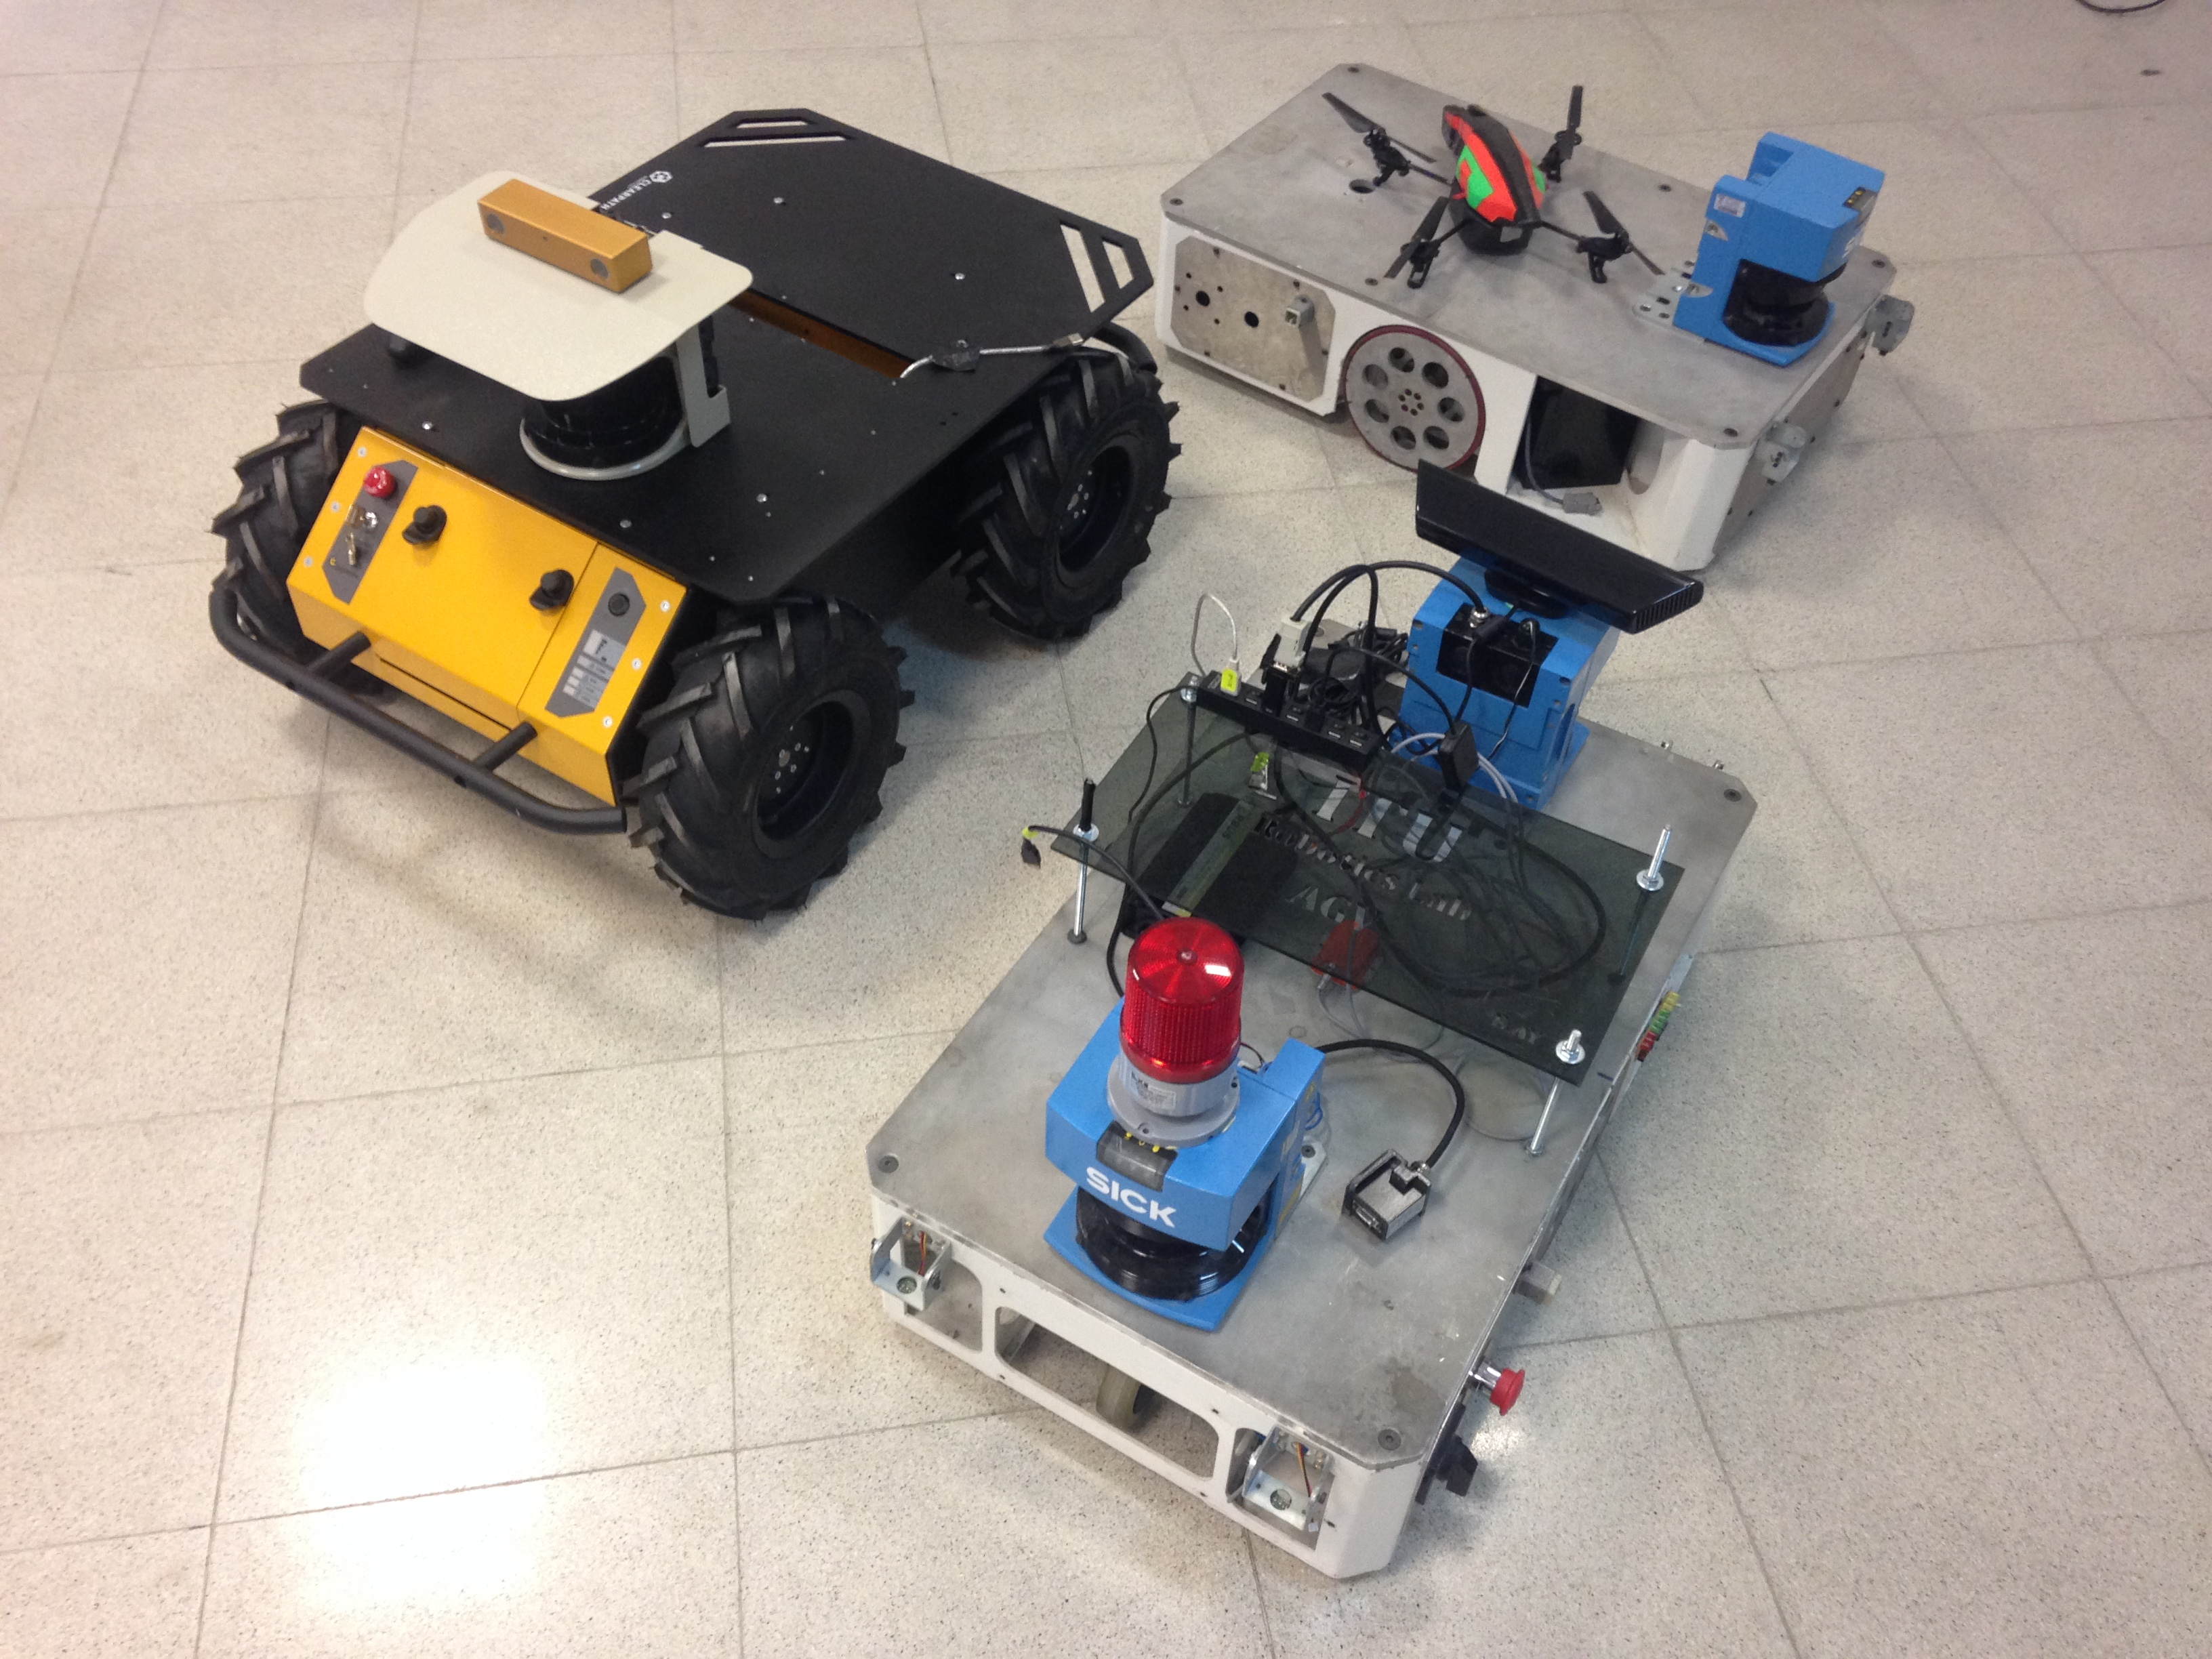
\includegraphics[scale=0.11]{images/husky}
		\caption{Husky robot, ITU-AGVs and AR Drone quadcopter at ITU Robotics Laboratory}
		\label{fig:husky}
	\end{figure}
\par
It is possible to develop autonomous applications based on this package. Navigation, SLAM, loop closure applications or swarm systems can be realized as well as heterogeneous robot groups. In ITU Robotics Laboratory, a group of robots are strategically gathered (Figure ~\ref{fig:husky}). A new outdoor robot kit Husky is bought and it is planned to work on with heterogeneous groups of Husky robot, AR Drone quadcopter and ITU-AGVs in outdoor or indoor, depending on the groups. ROS plays a significant role in the future projects and the package created in this project is the base step for this target. 

\appendix
\chapter{Codes \& Scripts}
\label{appendix}

The written codes of the indicated nodes are given in the appendix in order to avoid the interruption of the flow. Only selected codes and scripts are given in the appendix. All the written codes and scripts are available at;
\par
\centering
\url{https://github.com/emreay-/agv}

\lstinputlisting[language=c++,title={Odometry Broadcaster Node}]{codes/OdomTF.cpp}
\lstinputlisting[language=c++,title={Joint State Publihser Node}]{codes/jsPublisher.cpp}
\lstinputlisting[language=c++,title={Teleoperation Node}]{codes/agvTeleopnew.cpp}
\lstinputlisting[language=python,title={Node for sending the commands to LLPL}]{codes/agvSend.py}
\lstinputlisting[language=c++,title={Launch file for Teleoperation}]{codes/agvTeleopnew.launch}
\lstinputlisting[language=python,title={Node for getting encoder values from LLPL}]{codes/agvGet.py}



\backmatter

\bibliographystyle{plain}
\bibliography{refs}

\end{document}
